%Requires the memoir class 
\documentclass[oneside,12pt]{memoir}

%\usepackage{mathptmx}  % Times New Roman, but if you have Garamond then use it;
                        % you are writing a book, not a newspaper column

\DoubleSpacing        % memoir's double spacing
\usepackage{rice}     % rice thesis package 


\usepackage{graphicx}
\usepackage{rotating}
\usepackage{amssymb}

\usepackage{txfonts}  % I used this one to summon the symbol for \lambdabar
\usepackage{lmodern}

\usepackage[numbers,compress]{natbib}

\usepackage{hyperref}
\usepackage{memhfixc}

%%%% Definition of command shortcuts %%%%
\newcommand{\twos}[1]{\ensuremath{\hspace{-1pt}2\hspace{0.5pt}\hspace{0pt}S_{#1}\hspace{-1pt}}}
\newcommand{\twop}[1]{\ensuremath{\hspace{-1pt}2\hspace{0.5pt}\hspace{0pt}P_{#1}\hspace{-1pt}}}
\newcommand{\trep}[1]{\ensuremath{\hspace{-1pt}3\hspace{0.5pt}\hspace{0pt}P_{#1}\hspace{-1pt}}}

\newcommand{\cm}{\ensuremath{,\hspace{1pt}}}
\newcommand{\f}[1]{\ensuremath{F\hspace{-5pt}=\hspace{-4pt}#1}}
\newcommand{\mf}[1]{\ensuremath{m_{F}\hspace{-4pt}=\hspace{-4pt}#1}}
\newcommand{\mj}[1]{\ensuremath{m_{J}\hspace{-5pt}=\hspace{-4pt}#1}}
\newcommand{\mcm}{\ensuremath{\hspace{-4pt}}}

\newcommand{\red}{\ensuremath{ \twos{1/2}\hspace{-0.0pt}\rightarrow\hspace{-0.0pt}\twop{3/2} }\ }
\newcommand{\uv}{\ensuremath{ \twos{1/2}\hspace{-0.0pt}\rightarrow\hspace{-0.0pt}\trep{3/2} }\ }

\newcommand{\TD}{\ensuremath{ T_{D} }}
\newcommand{\TR}{\ensuremath{ T_{R} }}
\newcommand{\TF}{\ensuremath{ T_{F} }}

\newcommand{\one}{\ensuremath{|1\rangle }\ }
\newcommand{\two}{\ensuremath{|2\rangle }\ }

\newcommand{\isat}{ \ensuremath{ I_{\mathrm{sat}} } } 
\newcommand{\isatred}{ \ensuremath{ I_{sat\text{(red)}} } } 
\newcommand{\isatuv}{ \ensuremath{ I_{sat\text{(uv)}} } } 

\newcommand{\li} {\ensuremath{^{6}}Li\ }

\newcommand{\kb} { \ensuremath{k_{\mathrm{B}}}}


\DoubleSpacing

\begin{document}

\maxtocdepth{subsection}   % put everything into the ToC
\pagestyle{plain}          % pagestyle for the prelims

\frontmatter
\thetitlepage

%%%%%%%%%%%%%%%%%%%%%%%%%%%%%%%%%%%%%%%%%%%%%%%%%%%%%%%%%%%%%%%%%%%

% put your abstract here

\riceabstract
\pagestyle{empty}  % Rice requires no page numbering in the abstract
We have used the narrow \uv transition in the ultraviolet (UV) to laser cool
and magneto-optically trap (MOT) \li atoms.  Laser cooling of lithium atoms is
usually performed on the \red (D2) transition, where temperatures of twice the
Doppler limit, or $\sim$300~$\mu$K for lithium, are achieved.  The linewidth of
the UV transition is seven times narrower than the D2 line, resulting in a lower
Doppler limit.  We show that a MOT operating on the UV
transition reaches temperatures as low as 59~$\mu$K.  We load 6 million
atoms from this UV MOT into a 1070~nm optical dipole trap (ODT).  We show that
the light shift of the UV transition in the ODT is small and blue-shifted,
facilitating efficient loading.  Evaporative cooling of a two
spin-state mixture of \li in the ODT produces a quantum degenerate Fermi gas
with 3 million atoms in only 11 seconds.
\pagestyle{plain} % Restore page numbering.

% put your acknowledgements here 
 
\riceacknowledgements

This work was possible thanks to the support and guidance of my adviser Randy
Hulet.  James Hitchcock patiently taught me most of what I know about
experimental techniques in atomic physics and for that I will always be
indebted to him.  I am fortunate to get to think about physics alongside Russ
Hart, whose pragmatism and patience are as admirable as his keen eye for data.
Ernie Yang never ceases to surprise me with his fast learning ability and I
thank him for his numerous contributions to our experiment after only being
around for one year.  I wish to also acknowledge the contributions to the early
building of the experiment by Ted Corcovilos and the help I got from RQI summer
students Adrien Signoles, Florian Emaury,  Adam Reed, and Kevin Jourde.    I
wish to also acknowledge all other current and past lab members for making this
a better place to work.  I would also like to thank the members of my committee
for taking the time to review this work. 


%% \setdedication{ text } % if you want a dedication
%\ricededication

%\tableofcontents
\tableofcontents*  % The starred version does not add "Table of Contents" to the Table of Contents
                   % I prefer it this way


% I don't find these two particularly useful
%% \listoffigures  % if you want to include a list of figures  
%% \listoftables   % if you want to include a list of tables


%% if you have more prelim sections, then
%%%% \clearpage
%%%% \pagestyle{plain}
%%%% \prelimtitle   text % for sections after the ToC, etc, before main text


\mainmatter
\pagestyle{rice}


%% Change the spacing between paragraphs, I prefered this for readability 
\let\oldparskip\parskip
\setlength{\parskip}{0.8em}

\chapter{Introduction}

\chapter{Quantum Magnetism and The Fermi-Hubbard model}

\chapter{Realizing the Fermi-Hubbard model with ultracold atoms}


\chapter{Measurement techniques}

\section{Polarization phase-contrast imaging}

\section{Bragg scattering of light} 
 

\chapter{Experimental apparatus}

\section{Magneto-Optical Trap}
\section{Optical Dipole Trap}
\section{Compensated Optical Lattice}
\section{Bragg scattering setup} 


\chapter{Detection of antiferromagnetic correlations}

\chapter{Conclusion} 



%% finally, start of your main text
\chapter{Introduction}

A degenerate Fermi gas (DFG) of atoms was first produced in
1999~\cite{DeMarco1999}, four years after the first Bose-Einstein condensates
were produced~\cite{Cornell1995,Hulet1995,Ketterle1995}.  The reason for the
delay being principally that it is not possible to evaporatively cool identical
fermions in a magnetic trap. 

Evaporative cooling relies on rethermalization of the gas via elastic
collisions. For a long-range interaction potential\footnote{Atomic units are
used.  In atomic units, the electron mass ($m_{e}$), electron charge ($e$),
reduced Planck's constant ($\hbar$), and Coulomb's constant
($1/4\pi\varepsilon_{0}$) are unity by definition.   The atomic unit of length
is the Bohr radius, $a_{0}$, and the atomic unit of energy is the Hartree
$e^{2}/4\pi\varepsilon_{0}a_{0}$.   The mass of \li in atomic units is
$m=1.09\times 10^{4}$~a.u. } for a partial wave $\ell$, $\displaystyle
U(r,\ell) =\textstyle-\frac{C_{6}}{r^{6}} + \frac{\ell(\ell+1)}{Mr^{2}} $ and
the location and height of the centrifugal barrier are determined by \[
\frac{\partial U(r,\ell) }{\partial r}  = 0 \ \ \ \ \ \Rightarrow \ \  \ \ \
U_{\mathrm{cb}}(\ell ) = \frac{1}{3 (6\,C_{6})^{1/2}} \left(
\frac{\ell(\ell+1)}{M} \right)^{3/2}. \] For \li\mcm,
$C_{6}=1394~\mathrm{a.u}.$~\cite{Dalgarno1996}, and $\displaystyle
U_{\mathrm{cb}} (\ell)/\kb \approx (\ell(\ell+1))^{3/2}
\,\,\mathrm{mK}$.  At a temperature much less than $U_{\mathrm{cb}}(\ell)/\kb$,
atoms colliding with angular momentum $\ell$ do not have enough energy to
overcome the centrifugal barrier and their scattering phase shift, and hence
their scattering cross section, go to zero. Therefore, at low enough
temperatures only $\ell=0$ collisions can occur; however, for identical
fermions $\ell$ must be odd due to the required anti-symmetry of the
total wavefunction.   So when the temperature of a gas of identical fermions is
sufficiently far below $U_{\mathrm{cb}}(\ell=1)/\kb=2.8\,\mathrm{mK}$ the gas
becomes collisionless: $p$-wave collisions are thermally suppressed and
$s$-wave collisions are symmetry forbidden.   


This is not a problem when one confines fermions in different internal states
in a magnetic trap: the Pauli exclusion principle does not rule out $\ell=0$
collisions for distinguishable fermions.   However, when trapping fermions in
two different spin states, two-body inelastic collisions, can result in loss of
atoms or heating of the sample.   For fermionic $^{40}$K atoms there is a pair
of hyperfine states that are magnetically trappable and stable against spin
changing collisions.  It was with a mixture of these states that the first DFG
of atoms was produced~\cite{DeMarco1999}.   

For \li\mcm, the only other radioactively stable fermionic isotope among the
alkali, there are no pairs of internal states that are both magnetically
trappable and stable against spin changing collisions.    The suppression of
$s$-wave collisions forces the introduction of a second atomic species in order
to provide a colliding partner that will allow evaporative cooling to
degeneracy.  DFGs of \li have been obtained in this way using bosonic
$^{7}$Li~\cite{Truscott2001,Shreck2001}, $^{23}$Na~\cite{Hadzibabic2002}, or
$^{87}$Rb~\cite{Zimmermann2005} as a coolant.   


\section{All-optical production of degenerate quantum gases} 

All optical
production~\cite{Chapman2001,Granade2002,O'Hara2002,Weber2003,Jochim2003}
refers to experiments in which evaporative cooling is done in a far
off-resonance optical dipole trap, without magnetic trapping. Far-detuned
optical potentials can trap all ground states for a given atom, allowing
selection of ground states with favorable elastic and inelastic properties as
candidates to reach degeneracy.  In the case of Fermi gases, this offers the
ability to trap the two energetically lowest hyperfine sublevels (high-field
seekers), which are stable against spin changing collisions but are not
trappable in a magnetic trap.  This eliminates the need for sympathetic cooling
with another species and greatly simplifies the experimental setup.

Evaporative cooling in an optical trap is different than in a magnetic trap. In
a magnetic trap the tail of the Maxwell-Boltzmann distribution can be removed
without changing the shape of the trapping potential by using RF radiation to
drive transitions to untrapped states.  This leads to runaway evaporation,
where the density and the collision rate increase as the atoms get colder.  In
an optical dipole trap the intensity is reduced to force evaporation.  Reducing
the trap depth also lowers the confinement strength. This may lower the density
sufficiently to lower the collision rate, thus making evaporation less
efficient as it progresses \footnote{ Schemes to achieve runaway evaporation in
an optical trap have been demonstrated~\cite{Chin2008,Bouyer2009}, but they are
not as simple as just lowering the trap laser power.}.  This problem may be
mitigated by using a Feshbach resonance to increase the elastic collision cross
section.  In the case of bosons this must be done with care, as three-body
inelastic collisions can lead to rapid losses near a Feshbach resonance. For
fermions in a two-state mixture, three-body inelastic collisions are suppressed
due to the Pauli exclusion principle, but can become significant at high enough
densities~\cite{Du2009}.  The elastic collision cross section can reach the
unitarity limit\footnote{Near a Feshbach resonance the $s$-wave scattering
length diverges.  The scattering cross section, $\sigma=4\pi a_{s}^{2}$, cannot
go to infinity because this would violate conservation of the probability
current (unitarity), instead it takes the maximum allowed value which is
$4\pi/k^{2}$ for $s$-waves.} near the Feshbach resonance, leading to fast and
efficient evaporation to degeneracy.  

Optical traps thus provide a fast and very efficient way to evaporate spin
mixtures of fermions to quantum degeneracy;  however, they are not without
their challenges.   An essential prerequisite is a sufficiently deep optical
potential; the depth is determined by the temperature of atoms being loaded
into the trap.   Generally, the starting point for the production of quantum
gases is a magneto-optical trap (MOT).   For lithium and potassium  typical
temperatures achievable in a MOT are roughly twice the Doppler limit, or $300
\,\mu$K. Therefore, very large power or tightly focused optical traps are
required to efficiently transfer atoms from the MOT prior to evaporation.  

Quantum degenerate gases of \li have been realized using deep optical traps
loaded from a MOT.  To achieve the required trap depth, groups have used high
power lasers~\cite{O'Hara2002} or  resonator enhanced optical dipole
traps~\cite{Jochim2003}.  The approach that I present in this thesis involves a
moderate power 50~W fiber laser focused to a waist of 73~$\mu$m and relies on
narrow linewidth laser cooling of \li which can produce samples below 60~$\mu$K
in a MOT.

\section{Limit of laser cooling} 

The limit to the temperature of a laser cooled sample, in a two-level atom
picture, is the Doppler limit,  $\TD=\hbar\Gamma/(2\kb)$, where $\Gamma/(2\pi)$
is the natural linewidth of the excited state of the laser cooling
transition~\cite{Hansch1975,Wineland1975}.  In many cases, sub-Doppler cooling
can be achieved due to the multi-level character of real atoms and the limit to
cooling is then the recoil temperature, $\TR=\hbar^{2} k^{2}/ (2 m \kb)$, where
$k$ is the wave number of the laser cooling light and $m$ is the mass of the
atom. Polarization gradient cooling, the most widely used sub-Doppler cooling
method, is effective if the linewidth of the cooling transition is small
compared to the hyperfine splitting of the excited
state~\cite{Dalibard1989,Ungar1989,Weiss1989,Lett1989}.

% or if there is a large
%amount of magnetic degeneracy in the ground state of the atom~\cite{XuPRL2003}.  


For atoms like sodium, rubidium, or cesium polarization gradient
cooling~\cite{Dalibard1989,Ungar1989,Weiss1989,Lett1989}, provides samples with
temperatures on the order of $10 \,\mu$K.  For lithium and potassium, the
excited state hyperfine splitting is not well resolved and typical laser
cooling temperatures are $300 \,\mu$K.  At this temperature a deep optical trap
is required that can capture the atoms before forced evaporation to quantum
degeneracy. 

In our experiment we have realized a \li MOT operating on the narrow yet still
dipole allowed \uv transition (UVMOT). This transition has a Doppler limit of
20~$\mu$K and a recoil limit of 15~$\mu$K (see Fig.~\ref{fig:323levels}).   We
have achieved temperatures in the UVMOT as low as 57~$\mu$K.   This extra stage
of laser cooling reduces the intensity requirements of an optical dipole trap
for lithium and also provides a higher phase space density at the start of
evaporative cooling.  

\section{Outline of the thesis} 

In this thesis I start by describing the apparatus, which we refer to in the lab as
Apparatus3, and the various tools that have been implemented to make possible
the creation of a DFG.    Chapter~\ref{ch:uvmot} details the procedure used to
load the atoms into the UVMOT and shows results of measurements of the
properties of the UVMOT.  The all optical production of a degenerate gas
starting from atoms in the UVMOT is presented in Chapter~\ref{ch:alloptical}.
Finally in Chapter~\ref{ch:conclusion} the significance of our achievements is
summarized and the prospects for the future of Apparatus3 are laid out.  


%%%%%%%%%%%%%%%%%%%%%%%%%%%%%%%%%%%%%%%%%
%%%%%%%%%%%%%%%%%%%%%%%%%%%%%%%%%%%%%%%%% 
\chapter{Description of the apparatus}
\label{ch:desc}
%%%%%%%%%%%%%%%%%%%%%%%%%%%%%%%%%%%%%%%%%
%%%%%%%%%%%%%%%%%%%%%%%%%%%%%%%%%%%%%%%%%



The experiments described in this thesis take place inside a vacuum where the
pressure of the background gas is less than $5\times10^{-10}$~Torr.
Figure~\ref{fig:vacuum} shows the main components of the apparatus.   Atoms
from a thermal beam originating in the oven are decelerated by the Zeeman
slower and cooled transversally by the two-dimensional magneto-optical trap
(2DMOT)  before being captured in the magneto-optical trap (MOT) at the center
of the chamber, where the temperature can be as low as 300~$\mu$K.  We transfer
the atoms to the narrow linewidth magneto-optical trap operating on the
ultraviolet \uv transition (UVMOT) where they can be cooled to 57~$\mu$K.  From
the UVMOT we load an optical dipole trap where the atoms are evaporated to
quantum degeneracy.  Evaporation is performed in the presence of a bias
magnetic field of 330 G, where the scattering length is $\sim$ 280$a_{0}$.  We
perform evaporative cooling at 330~G instead of near the Feshbach resonance at
834~G because we observe density dependent loss in the unitary scattering
regime that is fast enough to reduce the efficiency of evaporation.  In the
following sections I describe the various parts of the system.  
\begin{figure}
\centering 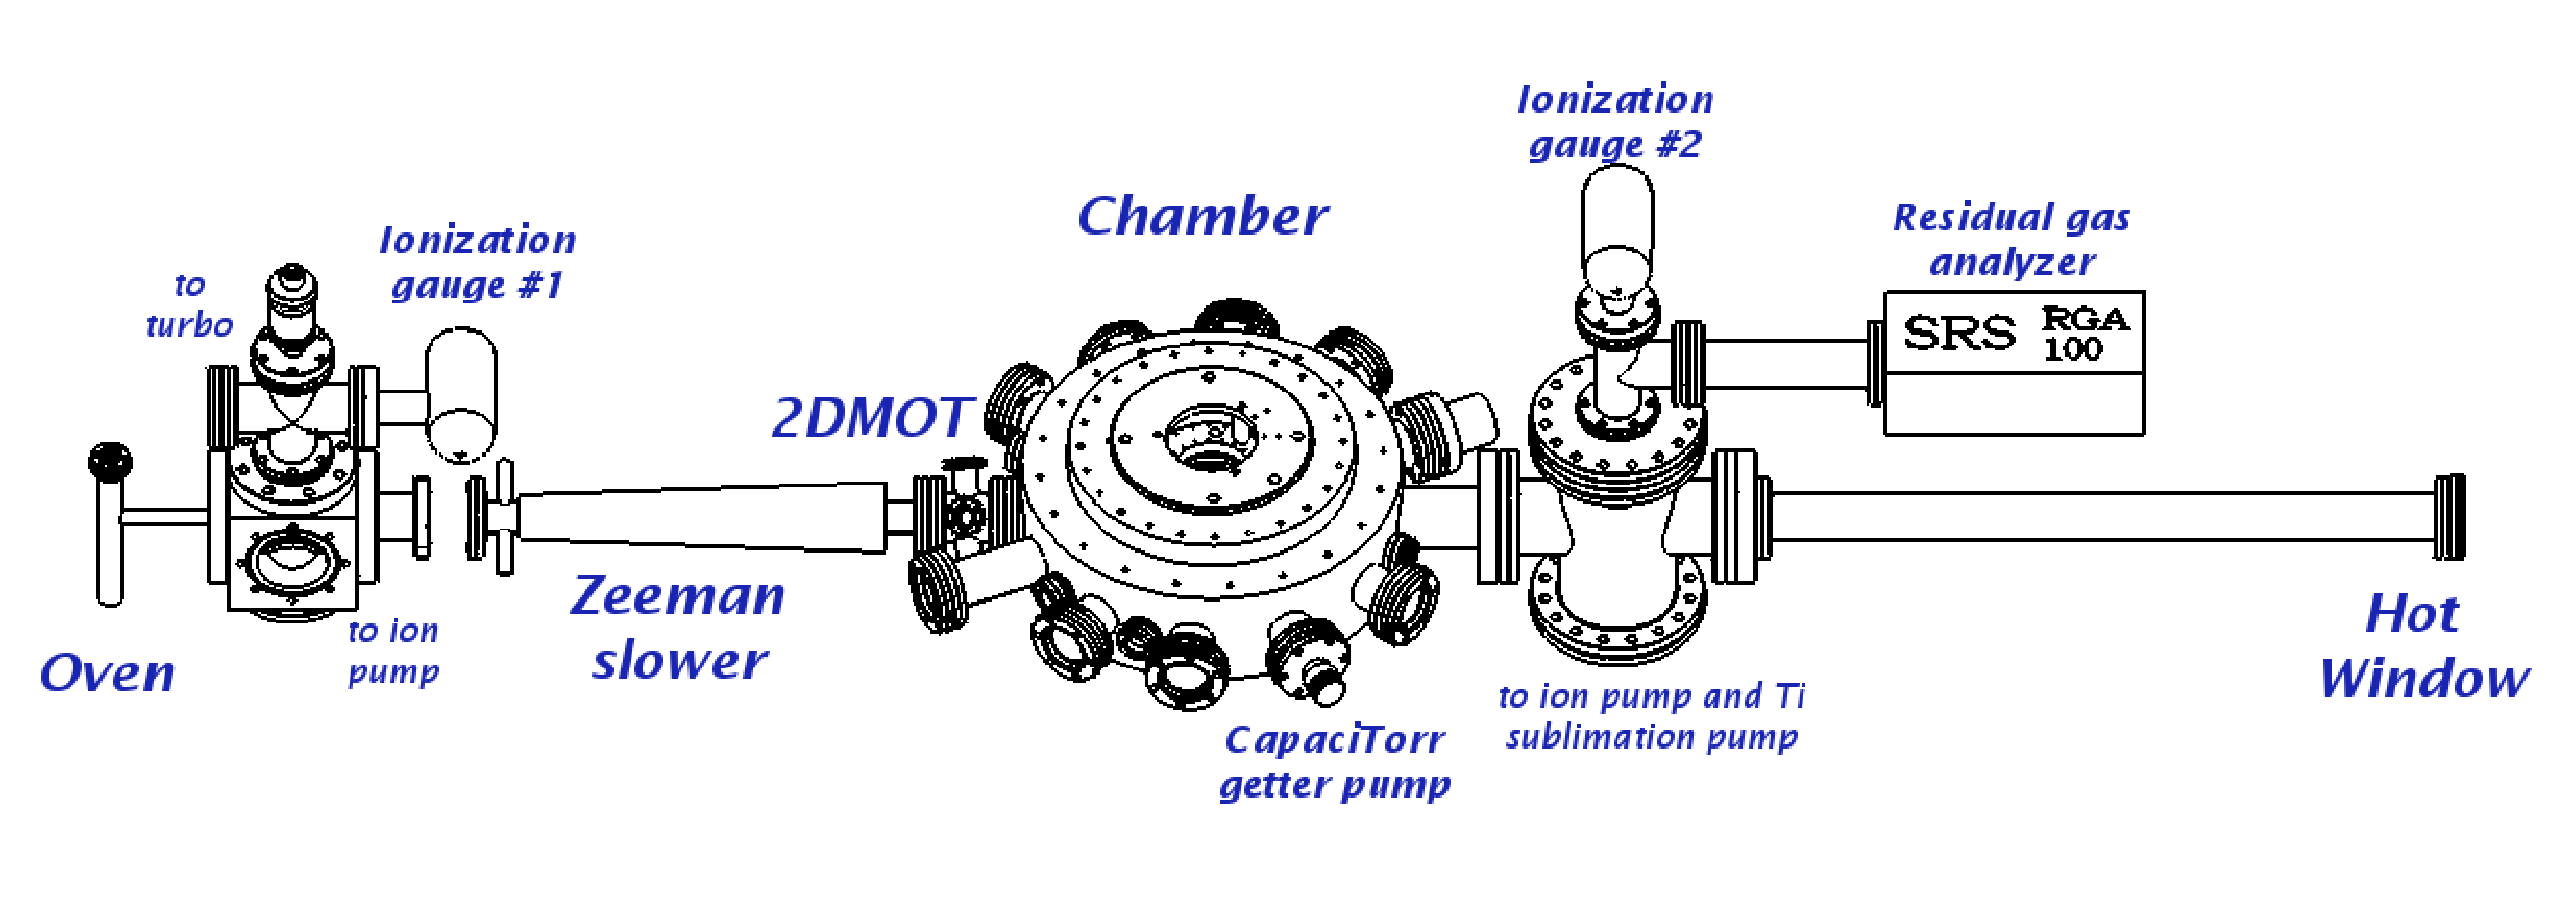
\includegraphics[width=\textwidth]{../figures/vacuum/vacuum02.pdf}
\caption[Apparatus3 vacuum system]{\small Main components of the Apparatus3
vacuum system.  Gate valves between the Zeeman slower and the oven region and
between the oven and the turbo pump are not shown. Ion pumps, titanium
sublimation pump, and turbo pump are also not shown.  } \label{fig:vacuum}
\end{figure}

%########################################
\section{Vacuum}
%########################################

During operation, the oven (see Fig.~\ref{fig:vacuum}) is heated to
450$^{\circ}$C to produce a collimated beam of lithium atoms.  The Zeeman
slower (see Sec.~\ref{subsec:zeemanslower}) is constructed with a narrow tube
and provides a low conductance (0.5~L/s) that can help maintain up to a factor
of 10 pressure differential between the oven and the main chamber sections.
The pressure\footnote{Measured with Bayard-Alpert type ionization gauge (Varian
Type 571) labeled \#1 in Fig.~\ref{fig:vacuum}} in the oven section is $4\times
10^{-9}$~Torr, and in the chamber section\footnote{Measured with ion gauge \#2}
is $5\times10^{-10}$~Torr.   

Lithium atoms that are not captured by the MOT eventually hit a sapphire
window, dubbed the `hot window', which is heated up to around 290$^{\circ}$C
to avoid coating it with the lithium metal.  The long tube between the chamber
and the hot window serves a differential pumping purpose;  the tube inside is
lined with a helical strip of non-evaporable getter material\footnote{SAES St
707/CTAM/30D, 30~mm wide strip.}.

The vacuum is maintained by two ion pumps and a non-evaporable getter pump.  A
VacIon Plus Starcell (150~L/s) from Varian vacuum technologies is connected to
the cross between the chamber and the hot window sections.   A titanium
sublimation cartridge is attached to this pump.  A smaller Vacion Plus Starcell
(55~L/s) is connected to the cube in the oven section.  A CapaciTorr B200
getter pump (90~L/s for H$_{2}$) is attached directly to one of the chamber
viewports.   Due to the close proximity of the getter pump to the atoms (8~cm)
we expect the background pressure to be lower in the center of the chamber than
the $5\times10^{-10}$~Torr measured with ion gauge \#2.

To initially pump down the system we have a TMU 071 turbo pump from Pfeiffer
Vacuum (50~L/s).  We currently keep this pump off because its vibration
introduces interference fringes in our absorption images.   A gate valve
between the cube and the turbo pump remains closed but can be opened if pumping
with the turbo pump is necessary.   Pumping continuously with the turbo pump
can reduce the pressure in the oven section by a factor of 2.   


%########################################
\section{671 nm Magneto-optical trap}
%########################################


The magneto-optical trap (MOT) in our experiment is a six beam MOT loaded from
a Zeeman slower plus a 2DMOT.   The light for the MOT, 2DMOT, and the Zeeman
slower is produced in a separate optical table and transferred to the apparatus
table in  optical fibers.  On the apparatus table, the MOT light is split into
six beams and the correct circular polarizations are set.  In this section I
describe the laser system used to produce the light for the MOT and the Zeeman
slower, and also give technical information about our Zeeman slower.  Details
about the operation parameters and characteristics of the MOT are deferred to
Chapter~\ref{ch:uvmot}.


%----------------------------------------
\subsection{Laser system}
%----------------------------------------

\begin{figure} \centering
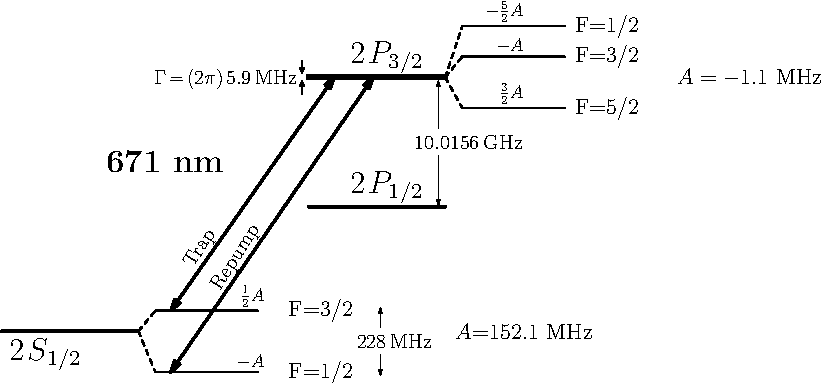
\includegraphics[width=0.95\textwidth]{../figures/levels/671-levels/lithium.pdf}
\caption[Lithium-6 energy level diagram]{\small Energy level diagram showing
transitions relevant for laser cooling \li using the \red transition. }
\label{fig:671levels} \end{figure} Efficient laser cooling relies on continuous
scattering of photons by the atom.  In a magneto-optical trap, a lithium atom,
see Fig.~\ref{fig:671levels}, that absorbs a photon on the
$\twos{1/2}\cm\f{3/2}\rightarrow\twop{3/2}$ transition, referred to as the
trapping transition, can decay to the
$\twos{1/2}\cm\f{1/2}$ state.  To maintain the continuous scattering of photons, a
second frequency that is tuned to the
$\twos{1/2}\cm\f{1/2}\rightarrow\twop{3/2}$ transition is required; we refer to
this transition as the repumping transition.  The probability of going to a
dark state is higher in lithium than in other alkalis such as rubidium, cesium,
or sodium  because the hyperfine structure of the excited state is unresolved,
$\Gamma\approx 5|A|$.  \begin{sidewaysfigure} \centering
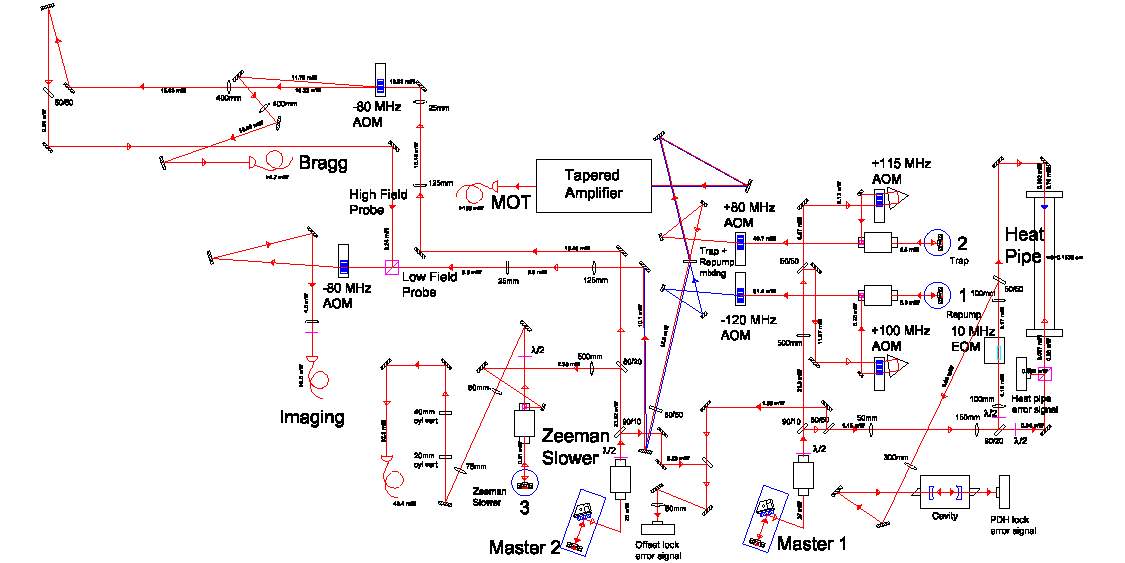
\includegraphics[width=1.\textwidth]{../figures/671setup/671setup(v4).pdf}
\vspace{1cm} \par \caption[671 nm laser system]{\small Intended for the in
house reader, this figure shows the layout of the Apparatus3 671 nm laser
system.  Benchmark powers are indicated on the figure.  } \label{fig:671system}
\end{sidewaysfigure} 

The laser system that is used to produce the trapping and repumping MOT light,
as well as the Zeeman slower and imaging probe light, is shown in detail in
Fig.~\ref{fig:671system}. We have two extended cavity diode lasers (ECDL),
which we refer to as MOT~Master and ZS~Master. The MOT~Master is stabilized to
the $\twos{1/2}\cm\f{3/2}\rightarrow\twop{3/2}$ transition via saturated
absorption spectroscopy (Fig.~\ref{fig:motmaster}) and the ZS~Master is
offset locked (red detuned) to the MOT~Master using the side-of-filter
technique~\cite{SoftLock2004} (Fig.~\ref{fig:zsmaster}).   The light from
the MOT~Master is split up for producing the trap and repump frequencies; each
path is passed through a double-pass acousto-optic modulator (AOM) which
injection-locks a slave laser diode used for amplification.  The trap and
repump light from the respective slaves are overlapped on a beamsplitter before
injecting a tapered amplifier.  The tapered amplifier output is fiber coupled
to the apparatus table. After passing through an AOM and splitting ten percent
of the light for the 2DMOT, we can get as much as 90 mW of power.   Due to the
small splitting between trap and repump frequencies, 22 mW of light are
produced by the tapered amplifier in unwanted sidebands at
\mbox{$f_{\mathrm{trap}}-228\,\mathrm{MHz}$} and
\mbox{$f_{\mathrm{repump}}+228\,\mathrm{MHz}$}~\cite{Ferrari1999}. This results
in a net 53~mW of trapping light and 16~mW of repumping light that are
dedicated to the MOT.  Besides the loss of power we have not observed negative
effects in the operation of the MOT from the presence of the sideband
frequencies created by the tapered amplifier.

The ZS~Master is used to produce the Zeeman slower light and the imaging probe.
Light from the ECDL is  split in two parts:  the first path injects a slave to
produce the Zeeman slower light, the second path is diverted to the imaging
setup.   The light from the Zeeman slower slave is coupled to an optical fiber
to be transferred to the apparatus table.   Light that goes to the imaging
setup is passed through an AOM and coupled to a fiber to be used as the probe
light for atoms at high magnetic field.   

\begin{figure} \centering
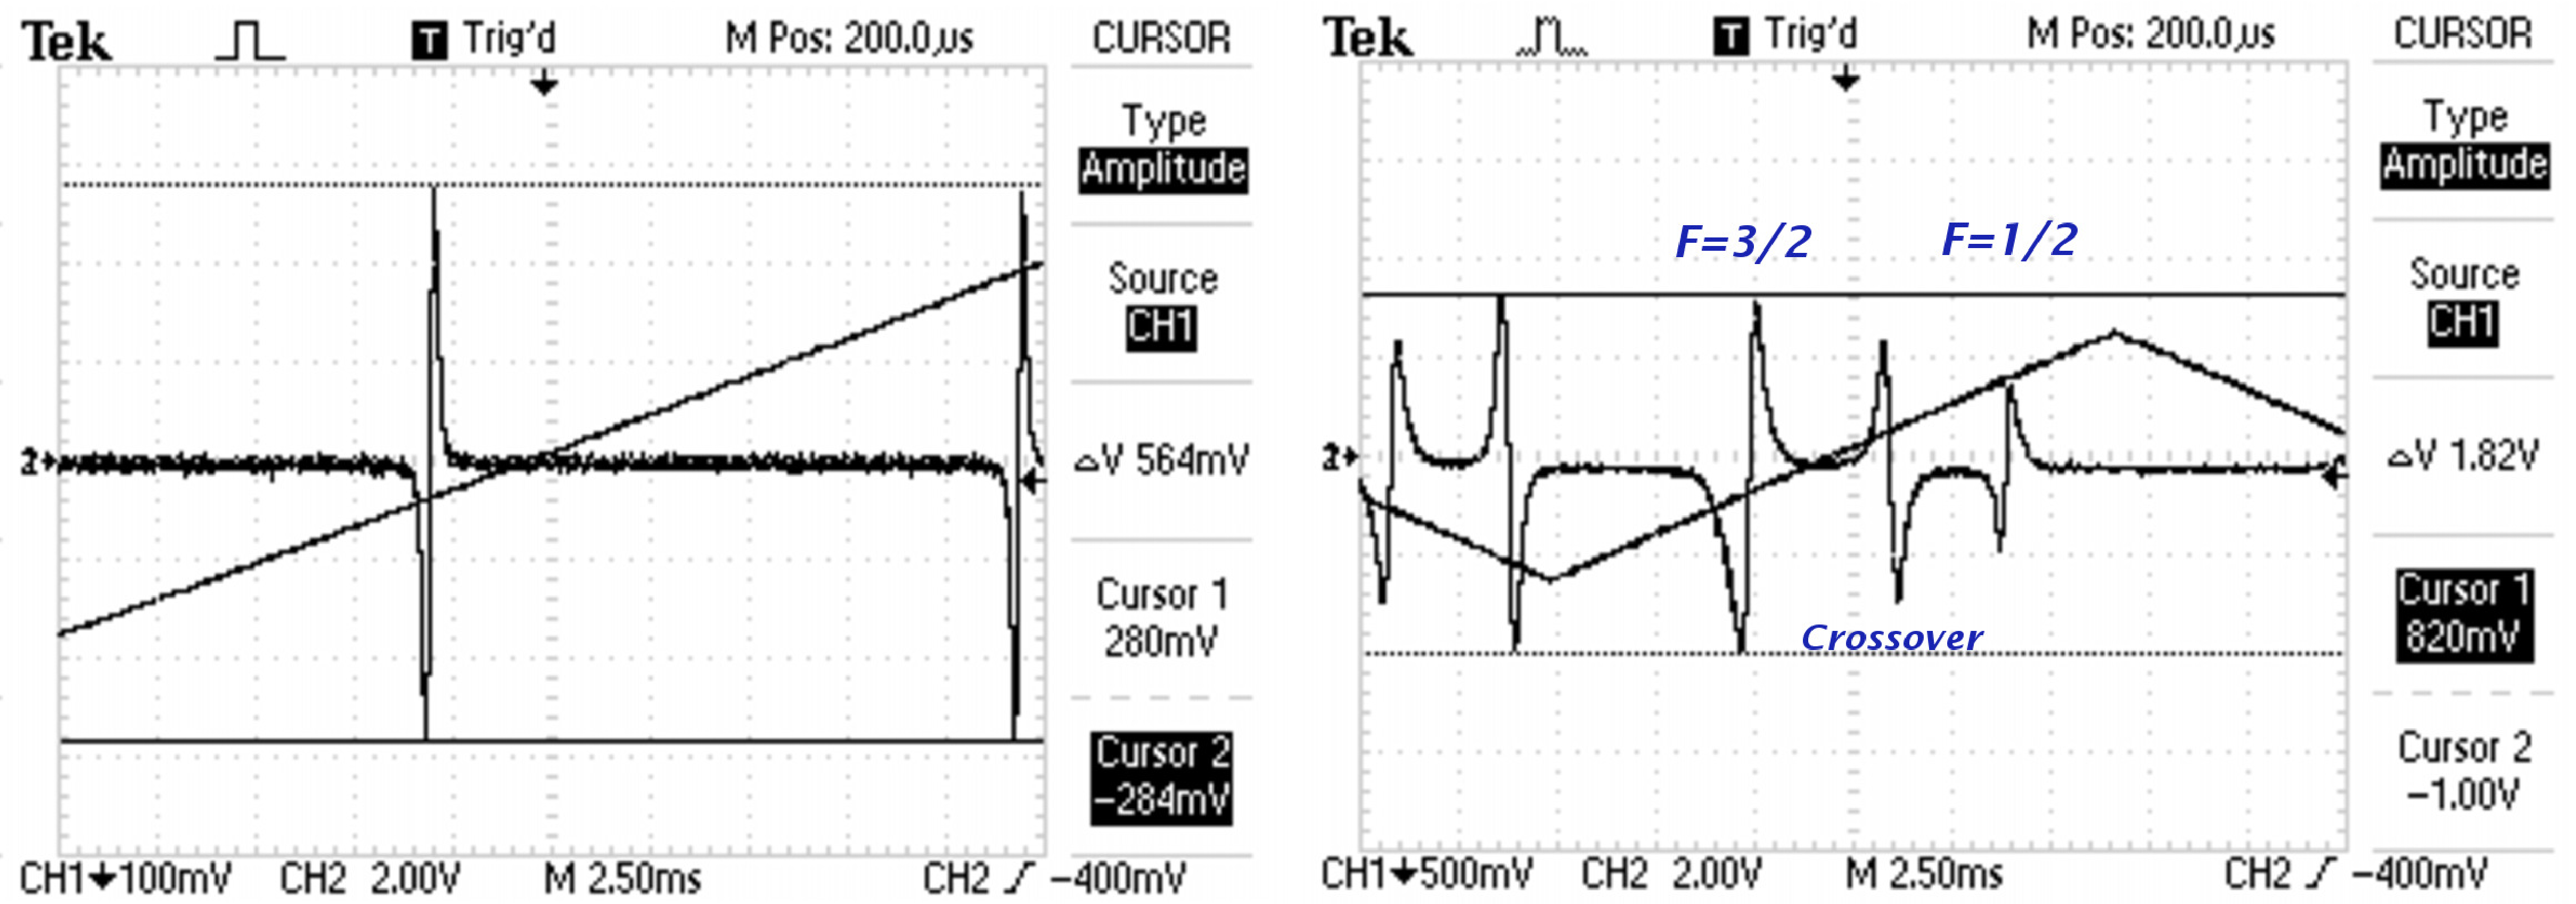
\includegraphics[width=0.95\textwidth]{../figures/671setup/MotMaster.pdf}
\caption[Lock error signals for  671 nm MOT~Master]{\small The MOT~Master is
stabilized to the error signal from a Fabry-Perot cavity (left). The cavity is
stabilized using a saturated absorption spectroscopy error signal obtained from
a lithium heat pipe.  To obtain both of the error signals shown in this figure
the Pound-Drever-Hall (PDH) technique is used, where the necessary sidebands
are produced by phase modulation with an electro-optic modulator at 13 MHz. }
\label{fig:motmaster} \end{figure}

\begin{figure} \centering
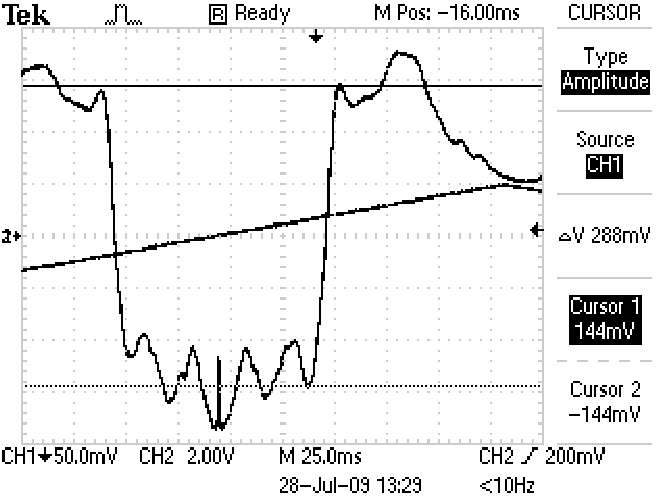
\includegraphics[width=0.475\textwidth]{../figures/671setup/offsetlock.pdf}
\caption[Side of filter lock error signal for 671 nm ZS~Master]{\small The
ZS~Master is stabilized using an error signal obtained using the side-of-filter
technique.   The zero crossing of the error signal is determined by the
frequency of a local oscillator which can be tuned.  In our setup we can tune
ZS~Master from -400 MHz to -1500 MHz with respect to  MOT~Master.  }
\label{fig:zsmaster} \end{figure}

	
%----------------------------------------
\subsection{Zeeman slower}
\label{subsec:zeemanslower}
%----------------------------------------
The Zeeman slower is effective in reducing the speed of atoms coming out of the
oven to less than the capture velocity of our MOT, $v_{\mathrm{c}}\simeq
5\Gamma/k = 20$ m/s, where $5\Gamma$ is the red detuning from resonance at
which we operate the MOT during loading. The Zeeman slower works by using red
detuned laser light propagating opposite to the lithium atomic beam.  Due to
the Doppler shift, the laser light is resonant with atoms coming out of the
oven, and via repeated photon scattering can produce a maximum deceleration
given by $a_{\mathrm{max}} = \frac{h\Gamma}{2\lambda m}$.  As the atoms get
slowed they shift out of resonance, but the magnetic field of the Zeeman slower
shifts the transition to the red keeping the atoms resonant with the light as
they travel through the slower.

The Zeeman slower operates on the $\sigma^{-}$  transition between the
$\twos{1/2}\cm\mj{-1/2}$ and $\twop{3/2}\cm\mj{-3/2}$ levels, shown in red in
Fig.~\ref{fig:zeemanlevels}. An advantage of choosing this transition is that
it is a cycling transition even at moderate magnetic fields.  This eliminates
the need for using repumping light in the Zeeman slower.  \begin{figure}
\centering
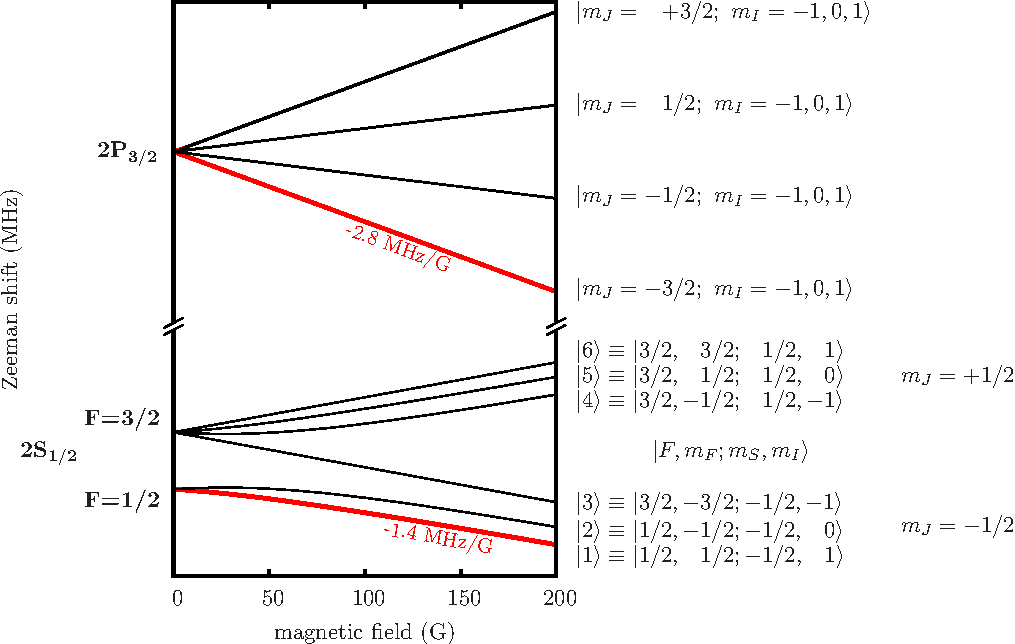
\includegraphics[width=1.0\textwidth]{../figures/levels/zeeman/01eps.pdf}
\caption[Levels of \li in a magnetic field. ]{\small Energy level diagram of
\li in a magnetic field.   The red lines show the levels used in the Zeeman
slower.  These levels are also used for absorption imaging, see
Sec.~\ref{subsec:absorption}. } \label{fig:zeemanlevels} \end{figure} We use a
detuning\footnote{This detuning is measured with respect to the \f{1/2} state.
Since the lock is referenced to the \f{3/2} state the reading on the frequency
counter of the offset lock is $1540-228=1312$~MHz.} of 1540~MHz, and a magnetic
field given by \[ B_{z} = B_{0}(1-\sqrt{1-z/L}) \] where $B_{0}\approx800$~G
and $L=34.5$~cm.   


%########################################
\section{323 nm Magneto-optical trap}
%########################################

In this section, I explain in detail the challenges encountered while setting
up the UVMOT and describe how we approached each of them; the main constraint
being the limited amount of power at 323 nm, which we obtain using a commercial
second harmonic generation (SHG) system from Toptica Photonics (see
Fig.~\ref{fig:shgsetup}).  


%----------------------------------------
\subsection{Laser frequency stabilization}
%----------------------------------------

A schematic of the setup for stabilizing the 323 nm light is shown in
Fig~\ref{fig:shgsetup}.  \begin{figure} \centering
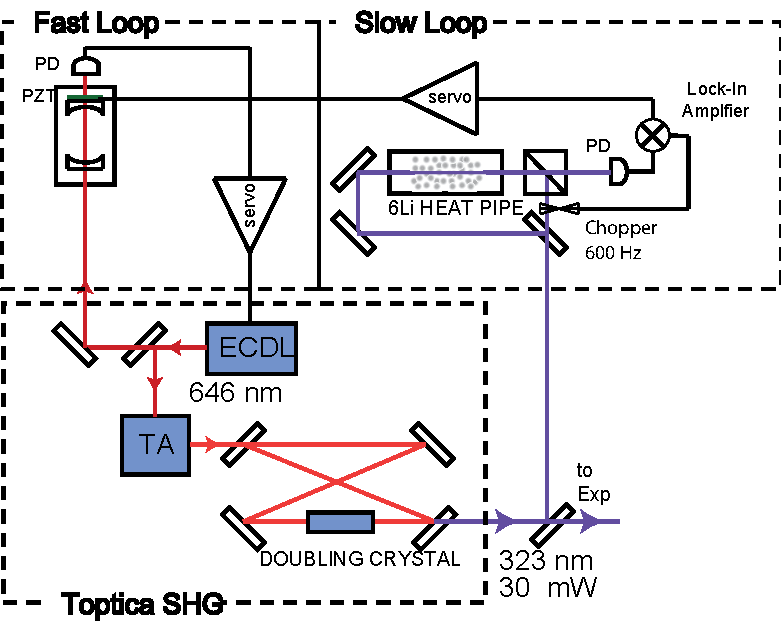
\includegraphics[width=0.5\textwidth]{../figures/323setup/323setup.pdf}
\caption[Schematic of stabilization setup for 323 nm laser]{\small The 323 nm
laser for the UVMOT is derived from a commercial TA-SHG system from Toptica
Photonics.  A 646 nm ECDL is amplified to 200 mW by a tapered amplifier.  Light
from the tapered amplifier is coupled to a doubling cavity which houses an
non-linear crystal to produce the frequency doubled light at 323 nm.  The
doubling cavity length is stabilized using the PDH technique.  The frequency
modulation sidebands are created by modulating the 646 nm diode laser current.
To stabilize the frequency of the 323 nm output, the 646 nm ECDL is first
locked to a Fabry-Perot cavity using the PDH technique.   The Fabry-Perot
cavity length is stabilized so that the doubled output is resonant with the
\,$\twos{1/2}\cm\f{3/2}\rightarrow\trep{3/2}$\, transition.  The error signal
to stabilize the cavity is obtained using  saturated absorption spectroscopy. }
\label{fig:shgsetup} \end{figure} With careful alignment, the SHG can put out
30 mW of light. The laser power slowly goes down with time, staying above 20 mW
for several months.  Whenever the power becomes less than 20 mW we go back and
perform a careful alignment of the doubling cavity.  On September 26  2011
Toptica upgraded our SHG system by installing a higher reflectivity incoupling
mirror in the doubling cavity.  This allowed us to increase the output power at
323 nm to 60 mW.  

The stabilization of the 323 nm light to the atomic resonance involves a fast
loop which locks the fundamental frequency to a Fabry-Perot cavity.   This
cavity is in turn stabilized using a slow loop so that the output of the SHG is
resonant with the $\twos{1/2}\cm\f{3/2}\rightarrow\trep{3/2}$ transition
(Fig.~\ref{fig:323levels}).   \begin{figure} \centering
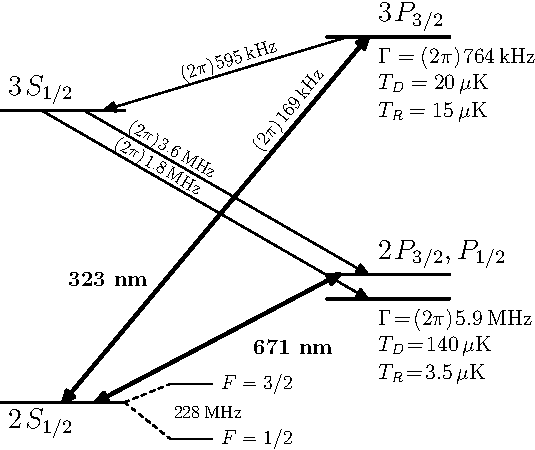
\includegraphics[width=0.75\textwidth]{../figures/levels/323-levels/lithium.pdf}
\caption[Lithium-6 energy level diagram showing the \trep{3/2} state]{\small
Lithium-6 energy level diagram. Lines in bold represent the transitions used to
laser cool atoms. Lighter lines represent decay pathways from the excited
\trep{3/2} state; the decay rates are indicated along the associated paths. }
\label{fig:323levels} \end{figure} 


%WRITE ABOUT THE CHARACTERISTICS OF THE FABRY-PEROT CAVITY
%EXPLAIN THE ORIGIN OF THE NOISE SEEN IN THE UV LASER POWER

Saturated absorption spectroscopy is used to obtain an error signal for
stabilizing the 323 nm laser. The error signal we obtain is shown in
Fig.~\ref{fig:323errsig}(a).  When the laser is locked to the \f{3/2}\ peak,
the rms linewidth is determined to be 210 kHz based on the observed noise and
calibrated slope of the error signal (Fig.~\ref{fig:323errsig}(b)).  In order
to obtain this error signal a saturated absorption setup is implemented with
only about 2 mW of light.  For this low power,  the  signal to noise ratio of
the spectroscopic feature is smaller  but then we can send  most of the power
to the experiment arm where it is used to create the UVMOT.  \begin{figure}
\makebox[0.5\textwidth][l]{(a)}\makebox[0.5\textwidth][l]{(b)} \centering
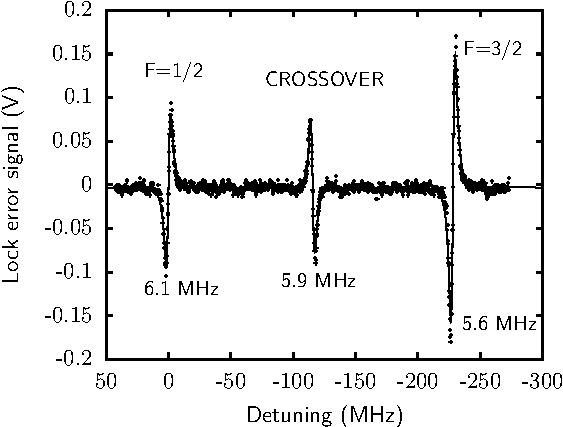
\includegraphics[width=0.49\textwidth]{../figures/323setup/heatpipe-errsig/errsigeps.pdf}
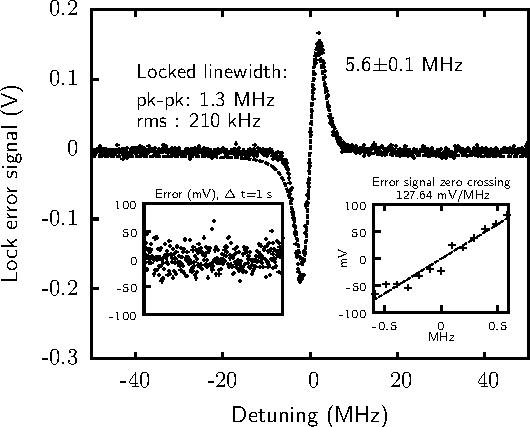
\includegraphics[width=0.49\textwidth]{../figures/323setup/trap-lockfig/lockfigeps.pdf}
\caption[323 nm saturated absorption spectrum]{\small (a).  Error signal used
to lock the 323 nm laser to the laser cooling transition. The indicated
linewidths are obtained from fits to the first derivative of a Lorentzian
profile.  (b). Close-up detail of the \f{3/2}\ peak.  The noise on the error
signal is shown when the laser is locked.  From this data, taken over 1~s at a
1~kHz sampling rate, the locked linewidth is estimated given the slope of the
error signal's zero crossing. } \label{fig:323errsig} \end{figure}


%----------------------------------------
\subsubsection{Modulation transfer spectroscopy}
%----------------------------------------

To obtain the spectroscopic signal shown in Fig~\ref{fig:323errsig} we perform
modulation transfer spectroscopy~\cite{ModTransfer2005}; a schematic of the
setup is shown in Fig~\ref{fig:modtransfer}\footnote{More details on the
electronics circuits built for this lock can be found in the undergraduate
thesis of Adam Reed who helped us build the lock during his internship in the
summer of 2010.}.    The frequency of the light is modulated using a
double-pass AOM.  The modulation depth is $\pm$1.5 MHz and the modulation
frequency is 35 kHz. The probe intensity,  measured with the photodiode shown
in Fig~\ref{fig:modtransfer}, is mixed with the modulation source to obtain the
derivative spectrum of the Bennett hole burn in the velocity distribution by
the pump beam.  In this way we are able to lock the laser to the zero crossing
rather than to the side of the feature.  

The main disadvantage of our setup is that we apply the frequency modulation
using the double pass AOM before splitting the pump and probe beams.  As a
consequence, the probe beam intensity has a small residual modulation at the
lock-in frequency of 35~kHz.  After mixing it with the modulation source, the
residual modulation shows in our error signal as an offset which can move the
zero crossing up and down in an uncontrolled way.   We get rid of this drifting
offset by using an optical chopper, shown in Fig.~\ref{fig:modtransfer} to
modulate the pump beam at 600 Hz.   The drifting derivative signal is mixed
with the chopper reference to obtain a stable spectrum which we use to lock the
323~nm laser.  
 
\begin{figure} \centering
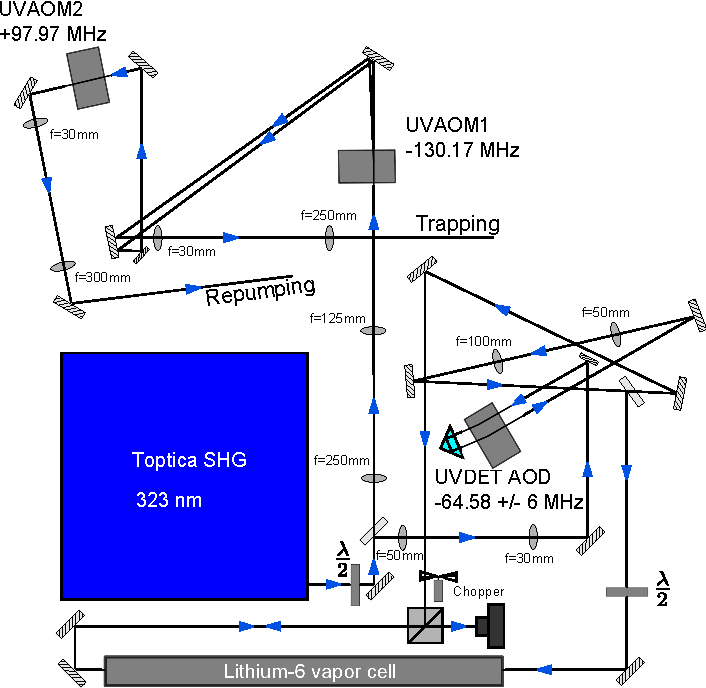
\includegraphics[width=0.7\textwidth]{../figures/323setup/aomsetup/optical_setup.pdf}
\caption[Schematic of modulation transfer spectroscopy]{\small Schematic
showing the optical setup for modulation transfer spectroscopy.   A double-pass
AOM is frequency modulated at 35 kHz.  The signal from the photodiode is mixed
with the modulation to obtain the modulation transfer signal.  An offset due to
residual amplitude modulation of the probe beam is removed by modulating the
pump with a mechanical chopper at 600 Hz.  The modulation transfer signal is
mixed with the chopper reference frequency to obtain the error signal showed in
Fig.~\ref{fig:323errsig}. The AOM's are labeled with their corresponding name
in the control program and the value of the frequency at which they are
nominally driven.   The driving frequency of the double-passed UVDET
acousto-optic deflector (AOD) provides the knob for the detuning of the light
used in the experiment.  The trapping and repump beams are combined using 50/50
beamsplitters and used in the experiment.} \label{fig:modtransfer} \end{figure}

We have observed that, if only the pump is modulated, the offset of the error
signal doesn't drift.  Unfortunately to implement such a setup we would need a
different combination of AOM's  to get the correct frequencies at the atoms.
For future reference, Fig.~\ref{fig:improved} shows a schematic of the setup if
improvements were to be done.
 
\begin{figure} \centering
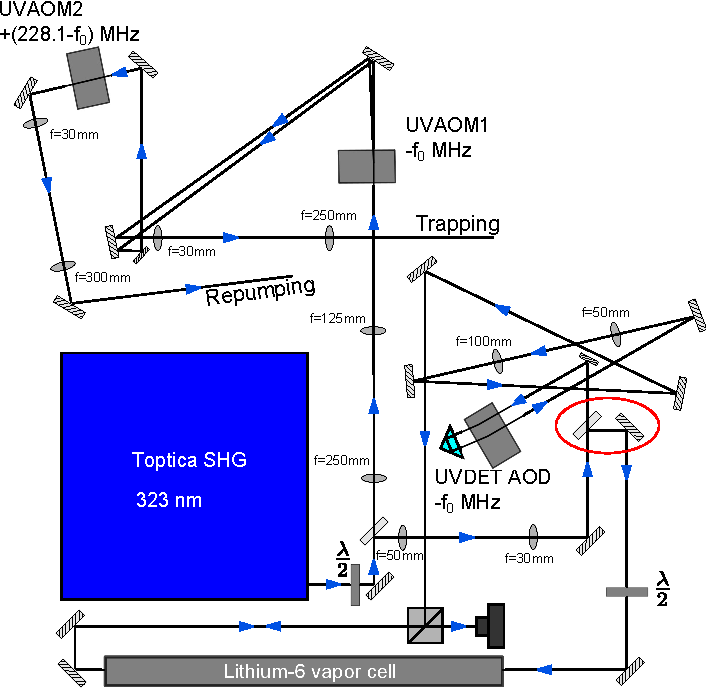
\includegraphics[width=0.7\textwidth]{../figures/323setup/aomsetup/improved_setup.pdf}
\caption[Improved AOM setup]{\small  By modulating only the pump beam there is
no need for a chopper to eliminate the error signal drift.  $f_{0}$ is the
driving frequency of the double-passed UVDET AOD.  The necessary frequencies
for UVAOM1 and UVAOM2 are indicated as a function of $f_{0}$. The red circle
emphasizes that the probe must be picked-off before passing through the UVDET
AOD.   } \label{fig:improved} \end{figure}

%----------------------------------------
\subsection{Vapor cell for saturated absorption spectroscopy}
%----------------------------------------

Constructing a vapor cell for spectroscopy of lithium is more difficult than
for cesium or rubidium, where an evacuated glass cell at room temperature can
do the job.   The vapor pressure for lithium is lower, making it necessary to
heat the lithium to more than 300$^{\circ}$C to achieve the required optical
density.  

In the lab we have built heat pipe ovens~\cite{HeatPipe1969} for doing
spectroscopy of lithium on the 671 nm transition.   A heat pipe oven can
provide a homogeneous vapor with a well defined optical density for doing
spectroscopy.  A heat pipe, as described in~\cite{HeatPipe1969,HeatPipe1971}
and shown in Fig.~\ref{fig:idealheatpipe}, works on the following basic
principles: \vspace{-0.5cm} \begin{itemize} \item  It has a capillary structure
on its inner surface.  This can be made with several layers of stainless steel
mesh.  The capillary structure serves as a wick: any lithium that condenses on
it is returned by capillary action to the central region, where it is heated to
create a vapor.  \item  It is filled with an inert gas.  The inert gas limits
the mean free path of the metal vapor so that it cannot reach and coat the
windows.  \end{itemize} \begin{figure} \centering
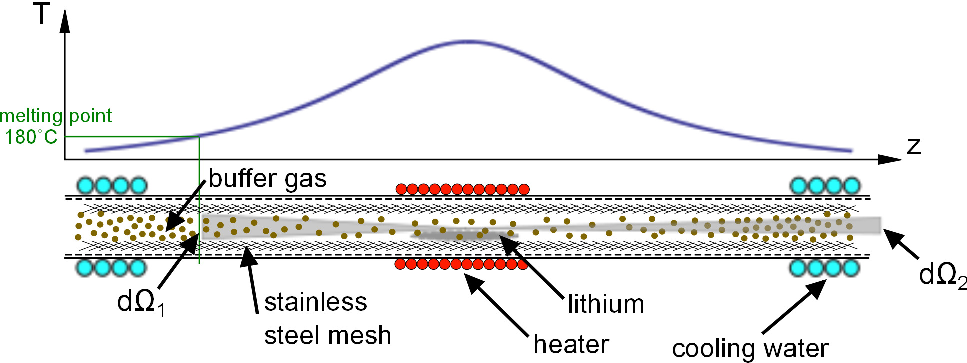
\includegraphics[width=0.7\textwidth]{../figures/323setup/heatpipe/idealheatpipe}
\caption[Schematic of a heat pipe oven]{\small Schematic of a heat pipe oven.
$\mathrm{d}\Omega_{1}$ is the solid angle for an atom to condense in a region
where it will not be wicked back to the center.  $\mathrm{d}\Omega_{2}$
represents the solid angle for an atom to reach the windows. }
\label{fig:idealheatpipe} \end{figure}

The original design of the heat pipe oven was meant for operation at high vapor
pressures of up to several Torr.  However, for doing saturated absorption
spectroscopy with relatively narrow linewidths one needs to evacuate the heat
pipe to pressures on the order of a few to a few tens of mTorr, otherwise the
resulting spectrum will be affected by pressure broadening~\cite{Olivares1998};
this includes the effect of velocity changing collisions which reduce the
signal to noise ratio of the Doppler-free spectrum.  We do not introduce  an
inert buffer gas at this pressures because the background gas\footnote{Most
likely hydrogen being outgassed by the stainless steel.} still provides a
buffer to protect the windows from getting coated. One also relies on the solid
angle $\mathrm{d}\Omega_{2}$ shown in Fig.~\ref{fig:idealheatpipe}, making it
small to minimize the possibility of lithium reaching the windows. 

The heat pipe that we used in Apparatus3 for spectroscopy on the 671~nm
transition had two design issues. First, only one layer of stainless steel mesh
was used. When only one layer of stainless steel mesh is used, any liquid
lithium that drips through it will be in contact with the stainless steel pipe
where capillary action is not effective in returning the liquid back to the
heated center. Second, the temperature profile of the pipe was unsuitable for
proper recirculation of the lithium via capillary action.    For ideal wicking
action the temperature profile of the pipe needs to be such that lithium is
evaporated preferentially from the center, as shown in
Fig.~\ref{fig:idealheatpipe}, and a long region of the heatpipe remains above
the melting point of lithium of 180$^{\circ}$C.  This minimizes the
accumulation of lithium in the regions that fall below the melting temperature. 


Given our constant issues with migration of the metal to the ends in the 671~nm
heat pipe, we tried a different design for the 323 nm~transition.  This design,
shown in Fig.~\ref{fig:323heatpipe}, does not have a stainless steel mesh to
act as a wick, and is therefore a vapor cell rather than a heat pipe. It is
made with a very narrow tube to minimize the solid angle for lithium to reach
the windows.   It was also made long, 71~cm, in an attempt to minimize the
timescale for migration of the lithium to the cold ends.    This heat pipe has
been working well and at the same temperature over one year\footnote{An
indication of lithium migration to the cold ends is that the temperature of the
center needs to be raised higher to maintain the same optical density.  This
means that one is raising the temperature profile to start evaporating metal
that has condensed further away from the center.}, so we think that this design
can provide a long term solution for our spectroscopic needs.  \begin{figure}
\centering
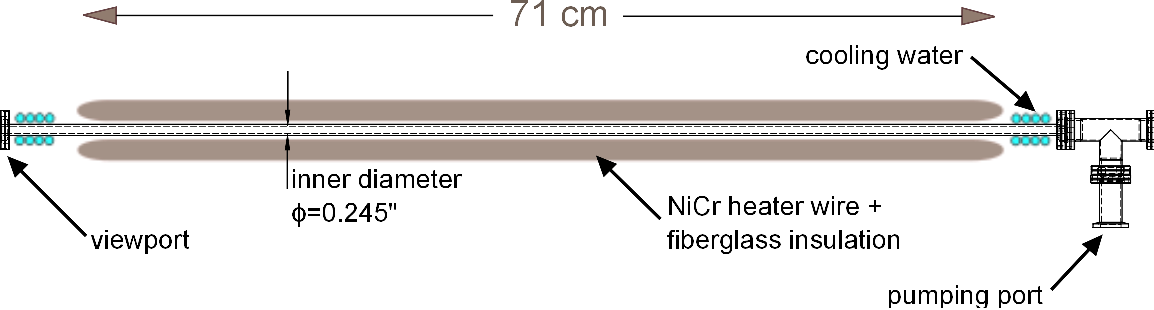
\includegraphics[width=\textwidth]{../figures/323setup/heatpipe/323heatpipe.pdf}
\caption[Vapor cell for the 323 nm transition]{\small Schematic of the vapor
cell used for saturated absorption spectroscopy on the 323~nm transition. }
\label{fig:323heatpipe} \end{figure} Future designs may want to incorporate
several layers of stainless steel mesh combined with an axially decreasing
temperature profile, in order to establish wicking.  A somewhat larger tube
diameter will be needed to accommodate the mesh. 


The spectrum obtained with the 323 nm heat pipe, which is shown in
Fig.~\ref{fig:323errsig}(a), is optimized at a temperature of 390$^{\circ}$C.
We observe, as it is expected~\cite{Olivares1998}, that the signal to noise
ratio of the spectroscopic signal is better for a lower background gas
pressure.  When pumped with a rotary vane pump\footnote{Edwards  DUO 5M,
pumping speed 1.7~L/s.} the background gas pressure can be as low as 2~mTorr.
However, after pumping is stopped, the pressure rises at a steady rate.   When
the pressure of the background gas goes above 25~mTorr the crossover peak is no
longer visible, and above 100~mTorr the \f{1/2} and \f{3/2} peaks have a signal
to noise ratio which makes them unsuitable for locking the laser. When this
pressure is reached we pump the heat pipe back to 2~mTorr again,  reducing the
temperature to 200$^{\circ}$ while it is being pumped to minimize risk of
coating the windows with lithium.   The rate of pressure rise at the present
day is about 0.5~mTorr/day, we have observed the rate gets smaller after every
subsequent pumping cycle.  

%----------------------------------------
\subsection{Beam waist and power balance}
%----------------------------------------

To choose the waist of  the UVMOT beams we had to take into consideration the
available laser power and the transmission losses on the viewports of our
apparatus, shown in Fig.~\ref{fig:012}, which are not anti-reflection coated at
323 nm.  \begin{figure} \begin{minipage}{0.5\linewidth}
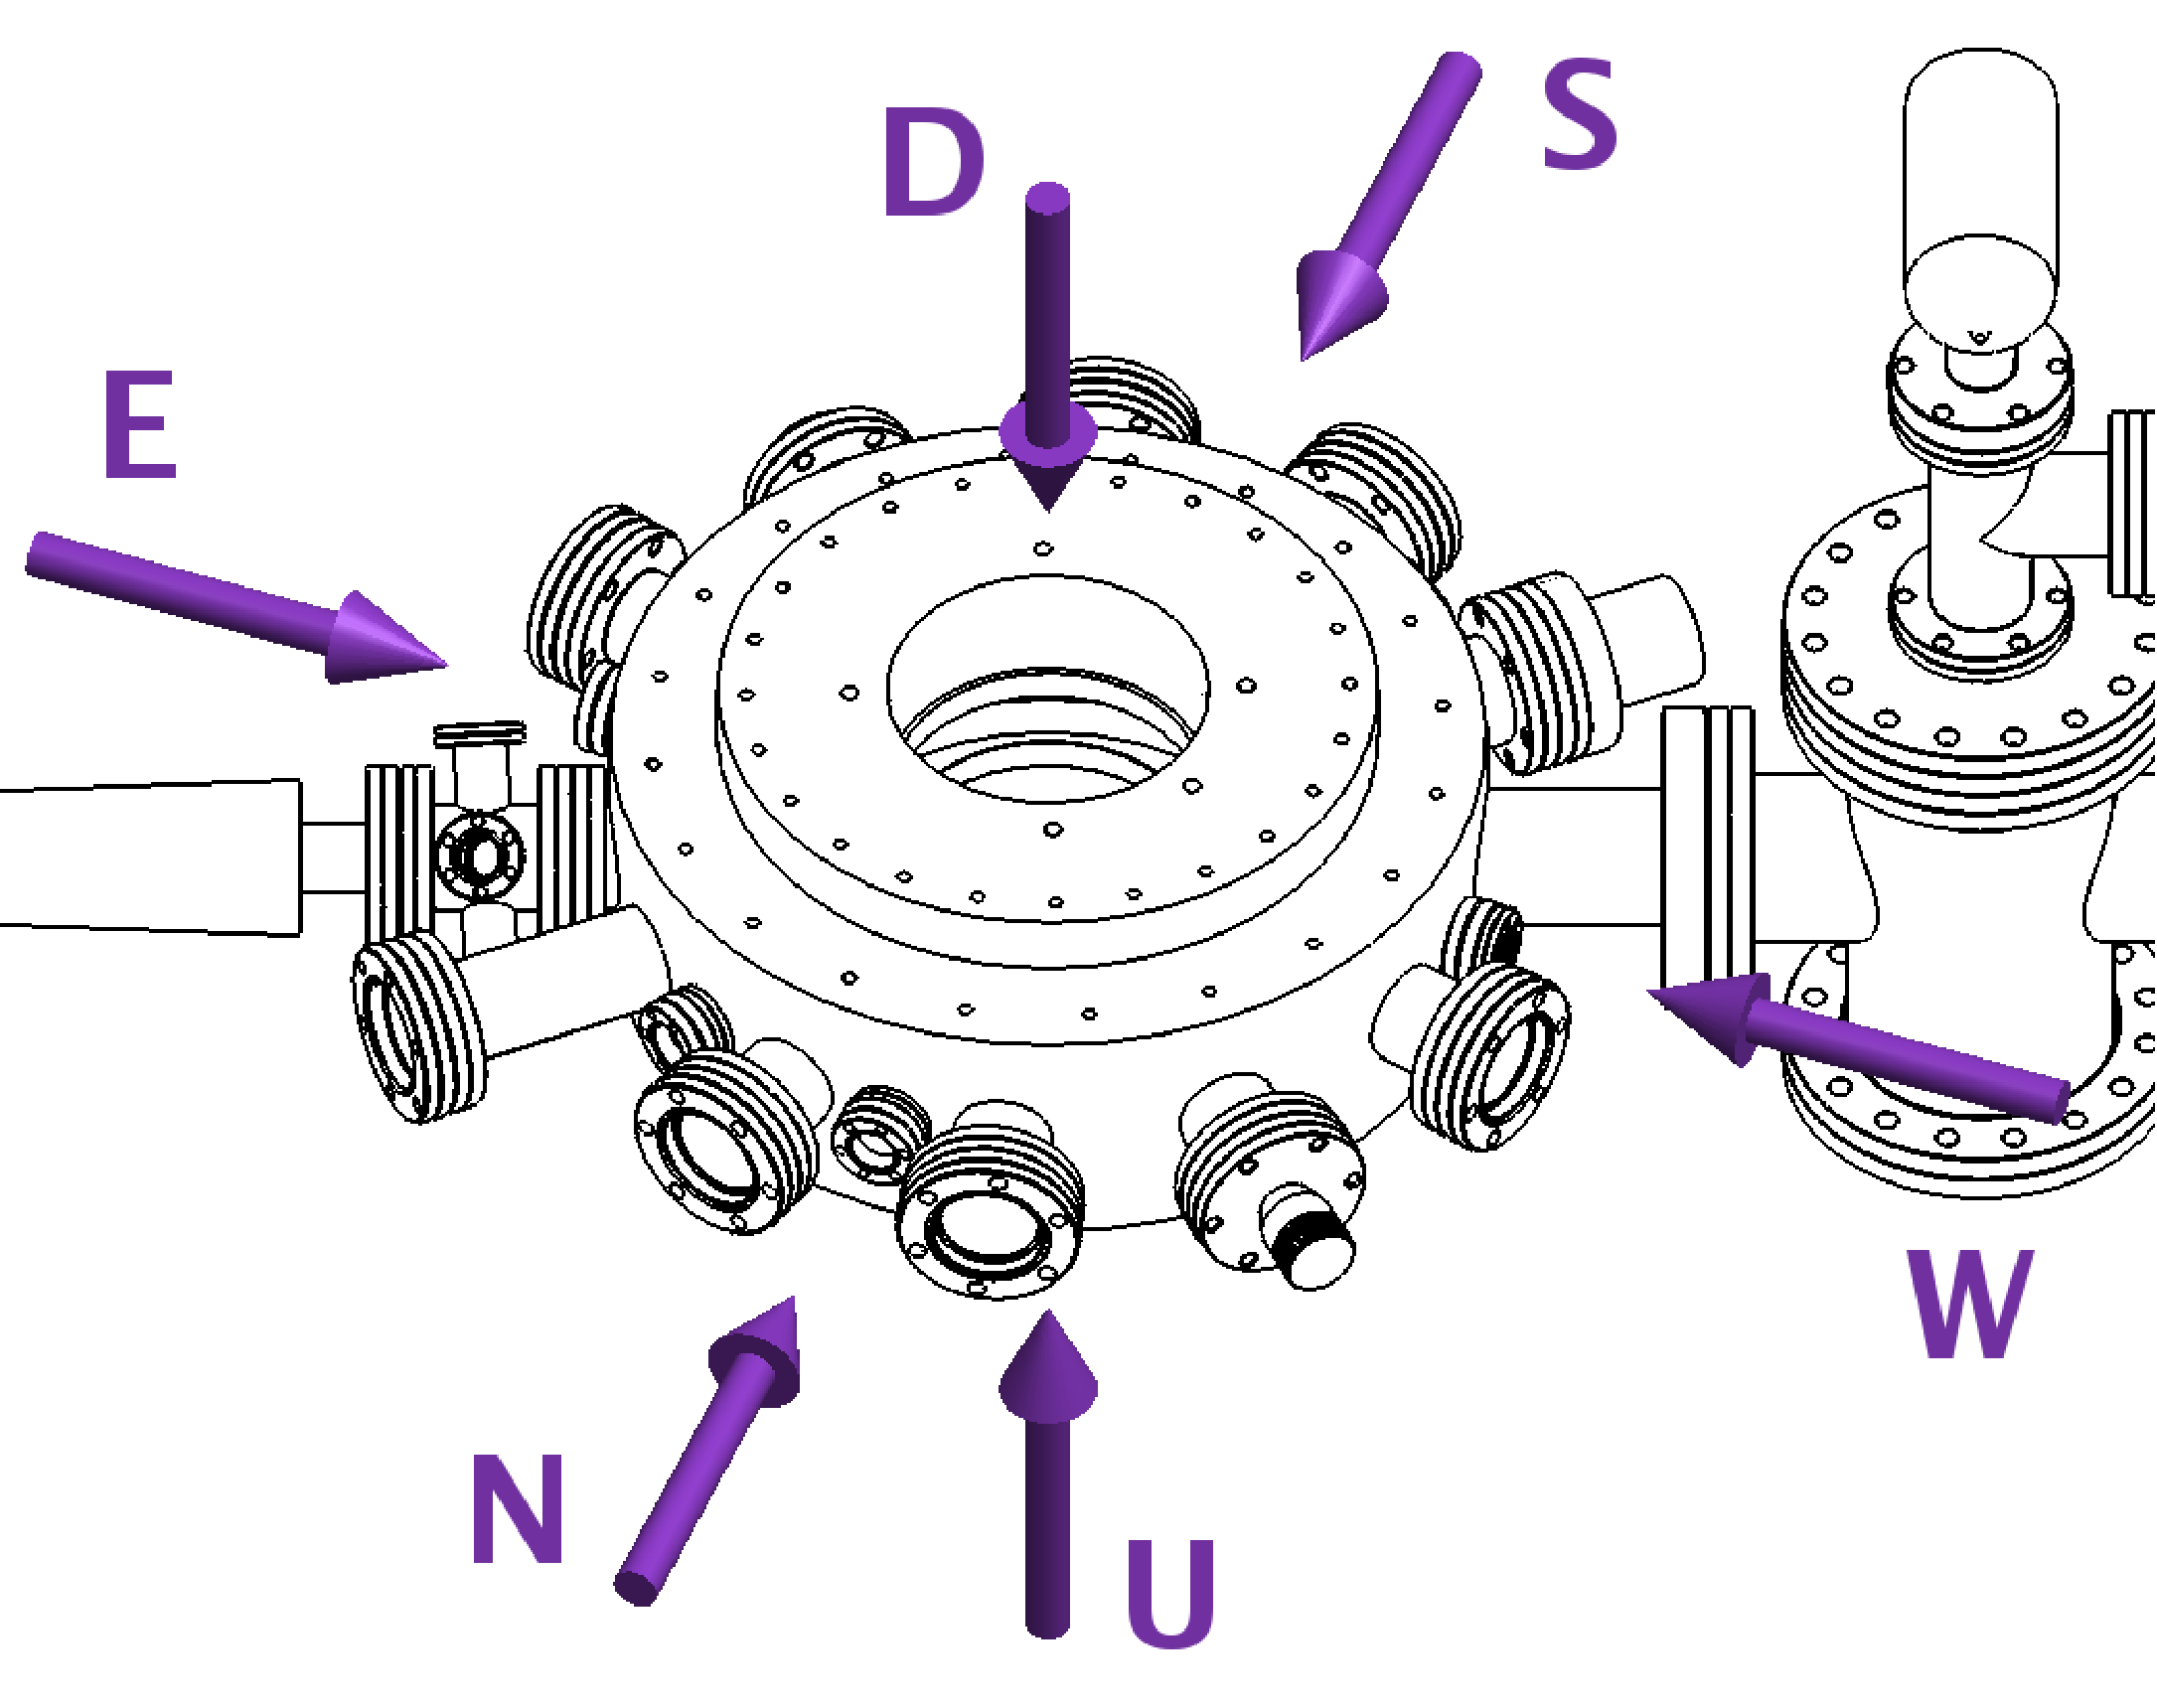
\includegraphics[width=\textwidth]{../figures/323setup/losses/losses.pdf}
\end{minipage} \begin{minipage}{0.5\linewidth} \centering \begin{tabular}{r|c}
& \% Transmission  \\ \hline N & 68 \\ S & 87 \\ E & 75 \\ W & 58 \\ U & 40 \\
D & 40 \\ \end{tabular} \end{minipage} \caption[UVMOT Losses on windows]{\small
This figure shows the percentage transmission of the 323 nm light through the
viewports on our vacuum chamber.  For the side viewports the losses were
accounted for by measuring the power reflected back by the window.  For the top
and bottom viewport it was harder to make this measurement due to restricted
access, so the square root of the transmission through both windows is used. }
\label{fig:012} \end{figure} We setup the beams so that they all have the same
intensity at the atoms, thus carefully taking into account the losses at each
window.  This was accomplished by varying the angle of incidence on dielectric
beamsplitters until the desired power ratio was achieved.  Polarization
beamsplitter cubes for 323 nm are expensive because they have to be optically
contacted.  We have observed that the UV light progressively damages the cement
used in lower priced polarizing beam-splitter cubes.  We did keep one
polarizing beam-splitter cube (not optically contacted) in our setup for doing
the first split of the UVMOT beams.  This allows some variability in the power
balance without having to realign the entire system.  Currently we loose 14\%
of the light on the mentioned cube.  Considering the losses at the windows and
the loss on the splitting cube we make the waist equal to 3.3 mm to achieve an
intensity of 1.0\isat per beam at an SHG output power of 27.4~mW.  

The UVMOT uses the same viewports as the 671 nm MOT. All six beams of both
wavelengths are overlapped by use of dichroic mirrors that transmit 671 nm and
reflect 323 nm.  We were lucky to find a long-pass filter (Part Num. NT64-634)
from Edmund Optics that, at very low cost per piece, provides $>99$\%
reflection at 323 nm and $>99$\% transmission at 671 nm for both S and P
polarizations at a 45$^{\circ}$ angle of incidence.  The UVMOT and red MOT also
share an axis with the optical dipole trap.  After the 671 nm and 323 nm are
combined they are overlapped with the optical dipole trap light using a
trichroic mirror (Custom made part from RMI Co.)  that reflects IR and
transmits visible.  The trichroic mirrors have $R>99.5$\% measured at 1064 nm
and 1070 nm,  $T=99$\% at 671 nm and $T=90$\% at 323 nm, all measured at a
45$^{\circ}$ angle of incidence.   In the future we will implement an optical
lattice which will share the top-bottom axis with the UVMOT and the red MOT; we
will use the trichroic mirrors there as well.


%########################################
\section{Optical dipole trap}
%########################################

In our experiment the optical dipole trap (ODT) is used to load atoms from the
UVMOT and then evaporatively cool them to degeneracy. The ODT has to be deep
enough to be able to capture sufficient atoms from the MOT. 

The light for the trap is provided by a broadband fiber laser operating at
1070~nm with an output power of 50~W.  Two beams crossing at an angle of
15$^{\circ}$ and with orthogonal polarizations form a crossed beam trap, see
Fig.~\ref{fig:odtsetup}.   The second pass shares an axis with the 671 nm and
323 nm MOTs; a trichroic mirror that reflects 1070 nm is used to overlap the
three wavelengths.  The beams are cylindrically symmetric and focused to a
$1/e^{2}$ radius of 73 $\mu$m.   The trap depth is given by \footnote{For
lithium a single beam of power $P$ and $1/e^{2}$ beam waist $w$ produces a
trap with a depth $U=\frac{P}{w^{2}} \times 38.7\times10^{3}  \mathrm{\mu K\,
\mu m^{2}\, W^{-1}} $ .} \[ U_{\mathrm{dip}}(\mathrm{\mathbf{r}} ) =
\frac{\hbar \Gamma^{2}}{4} \left( \frac{1}{\omega_{0}+\omega} +
\frac{1}{\omega_{0}-\omega} \right) \frac{I(\mathrm{\mathbf{r}} )}{\isat} \] 

The first pass through the atoms has 39 W of power and after losses at the
optics and windows there are 35 W for the second pass.  This gives a trap depth
of 280 $\mu$K and calculated trap frequencies of 491 Hz, 3728 Hz, and 3760 Hz.
We measured the radial trap frequency by turning the dipole trap off briefly
(40 $\mu$s) and then turning it back on. The resulting breathing mode
oscillates at twice the trap frequency and we obtain $\omega_{\mathrm{r}} =
(2\pi)3.8$~kHz.   The axial trap frequency was measured via parametric heating
by sinusoidally modulating the trap depth.  The number of atoms after
modulation shows a loss  resonant centered at twice the trap frequency.   In
this way we determined the axial trap frequency to be 1/8 of the radial trap
frequency, or $\omega_{\mathrm{a}} = (2\pi)475$~Hz.  


In order to correct for any astigmatism on the beam  a CCD camera was used to
take pictures of the beam profile. The lenses labeled $E$ and $T$ on
Fig.~\ref{fig:odtsetup} are mounted on gimbal mounts and can be tilted to
correct for the astigmatism in the first and second waist respectively.
Changing the separation between lenses $E$ and $F$ provides a very sensitive
handle on the beam waist and it is what we used in the end to set it to the
value that we desired.  \begin{figure} \centering
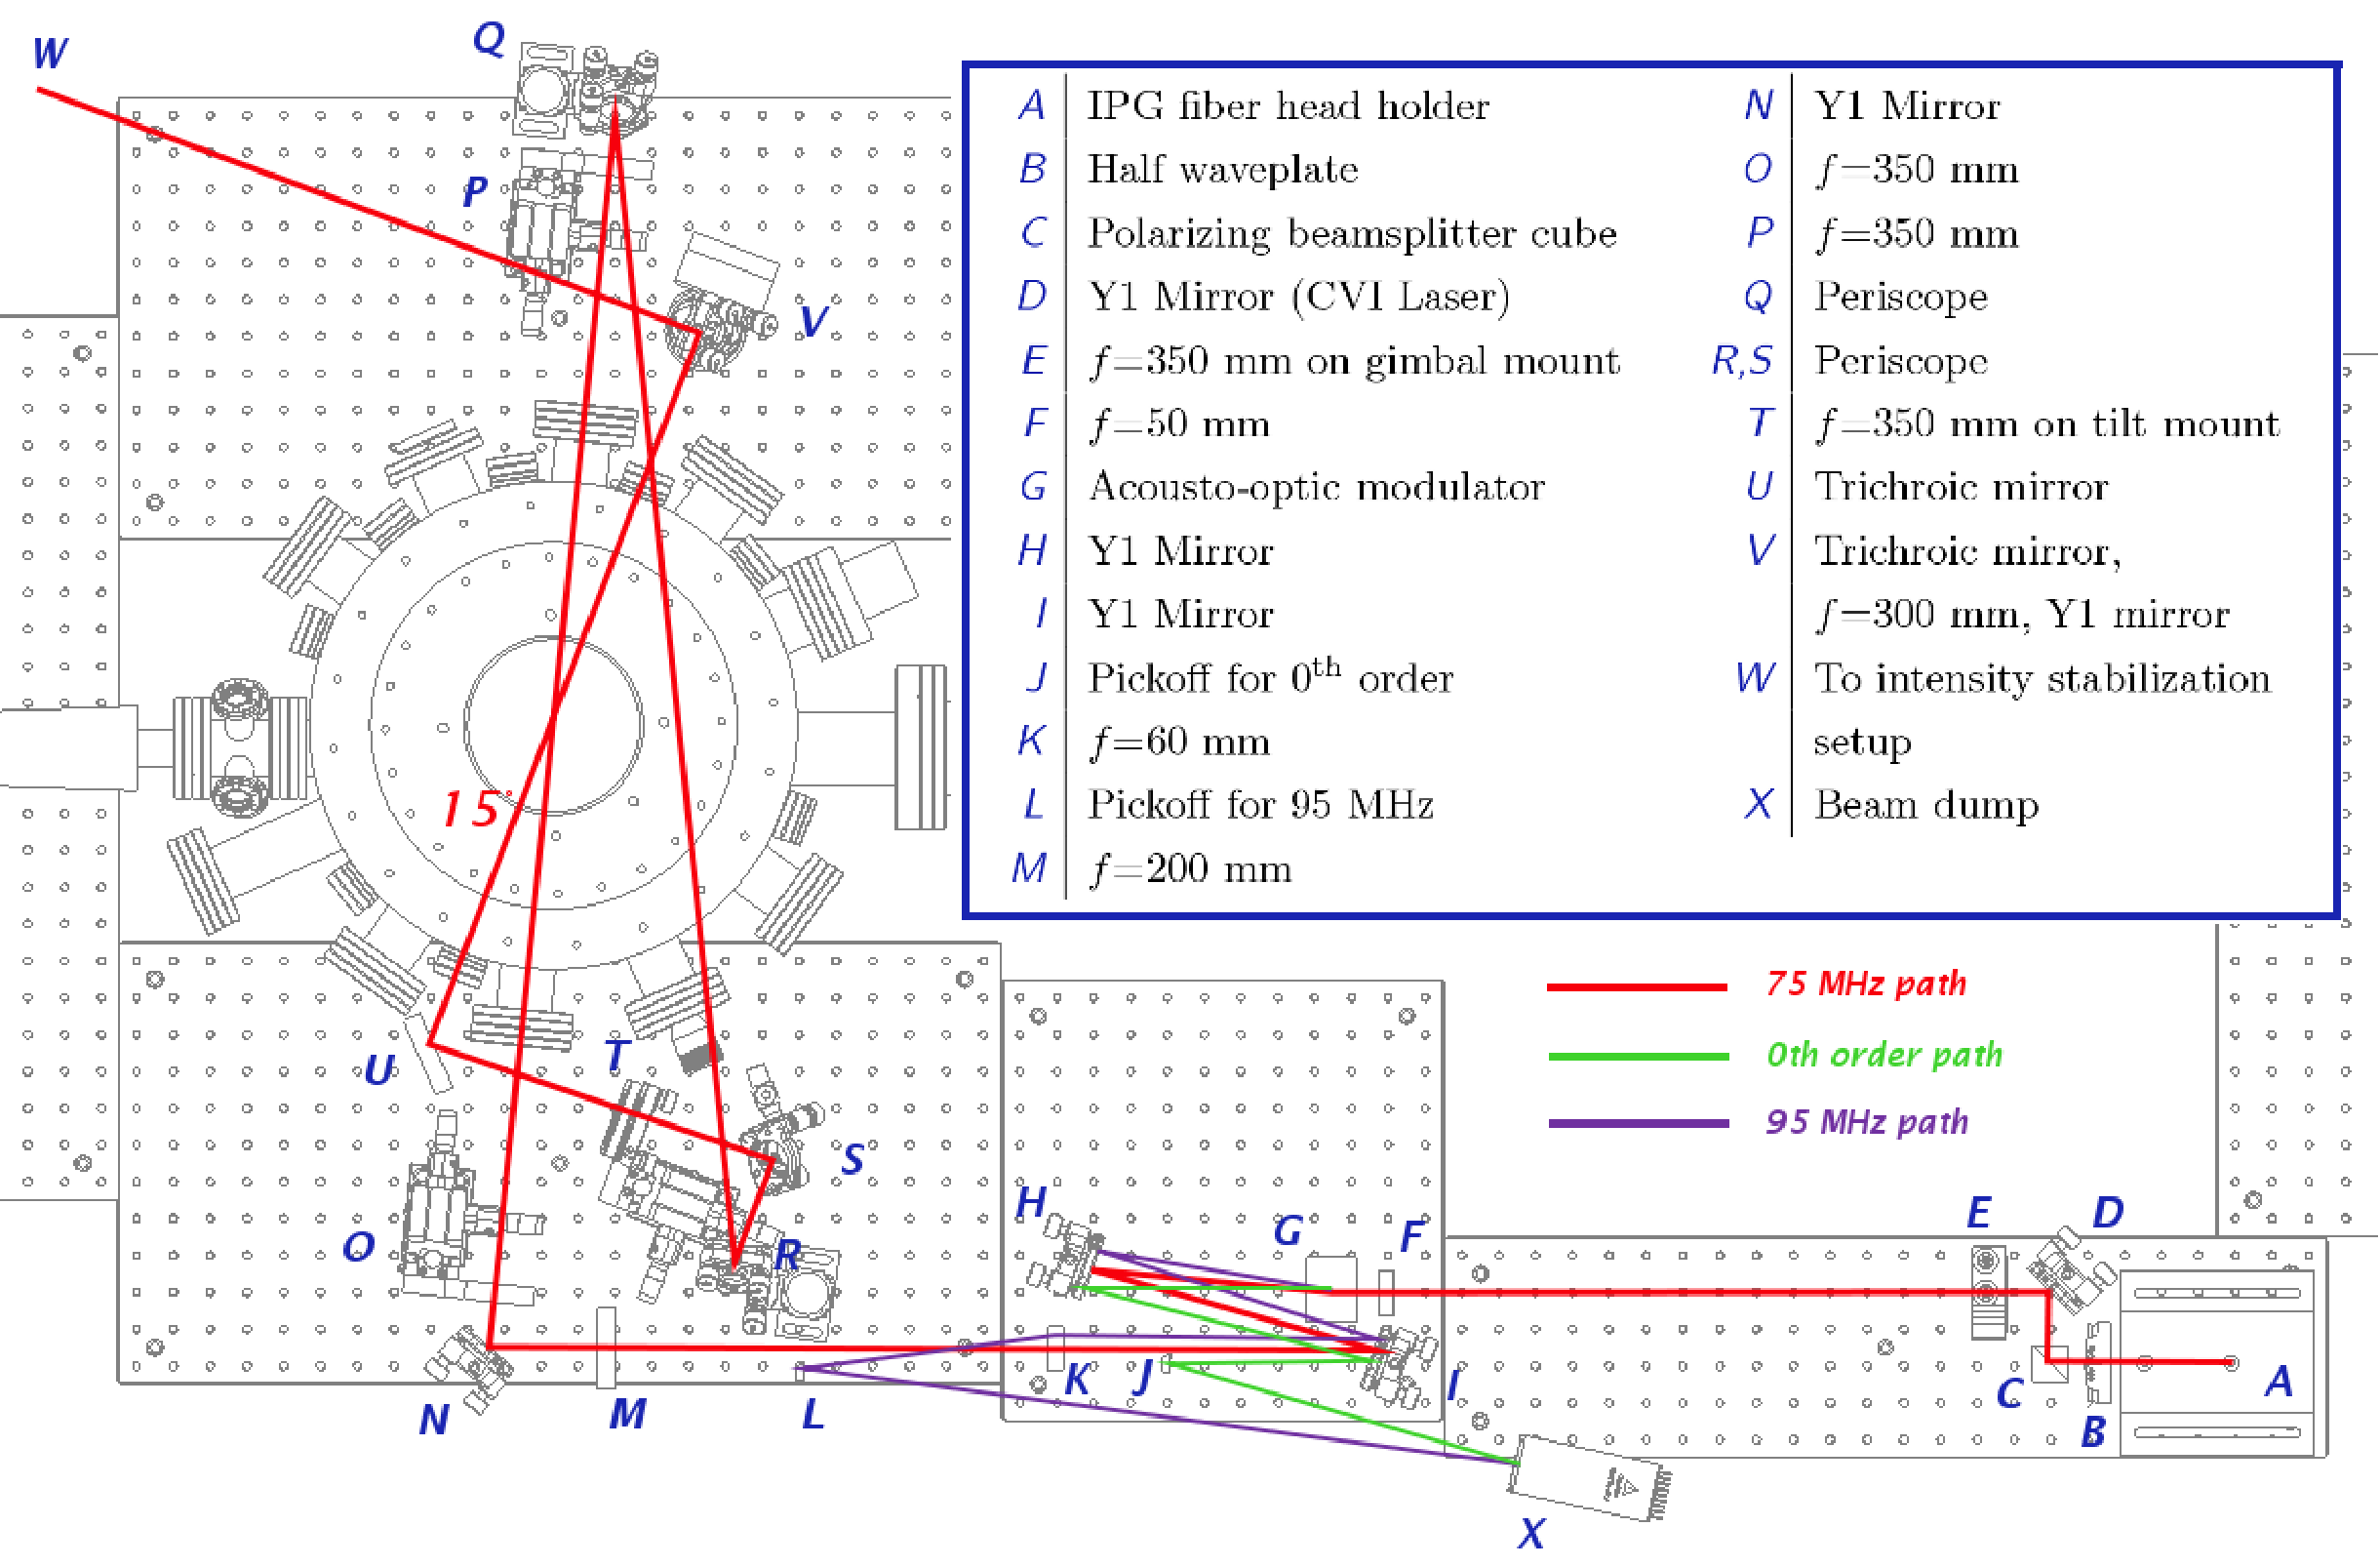
\includegraphics[width=\textwidth]{../figures/odt/opticalsetup/setup.pdf}
\caption[Optical dipole trap setup]{\small Optical dipole trap setup.  The AOM
can be off (green), at 75 MHz (red), and at 95 MHz (purple).  For the mirrors in
this setup we used Part Num. Y1-1025-45-UNP from CVI Laser, which have a damage
threshold of 10~MW/cm$^{2}$.  All the lens substrates are UV fused silica to
reduce power dissipation and thermal lensing.  The acousto-optic modulator is
Part Num.  46080-2-1.06 from Neos Technologies.  } \label{fig:odtsetup}
\end{figure}

In order to avoid thermal drifting of the position of our dipole trap we try to
keep maximum RF power on the AOM at all times.  During operation, the AOM is
driven at 75 MHz.  Otherwise the AOM is driven at a frequency of 95 MHz, the
diffracted beam is picked off from the main path and sent to a beam dump.  The
undiffracted 0$^{\mathrm{th}}$ order is sent to the same beam dump as shown in
Fig.~\ref{fig:odtsetup}.   


%########################################
\section{Magnetic field}
%########################################

The magnetic field in our experiment is created by a set of coils in
Helmholtz configuration that are close to the atoms, inside the recessed top
and bottom viewports of our vacuum chamber (Fig.~\ref{fig:coilforms}).
\begin{figure} 
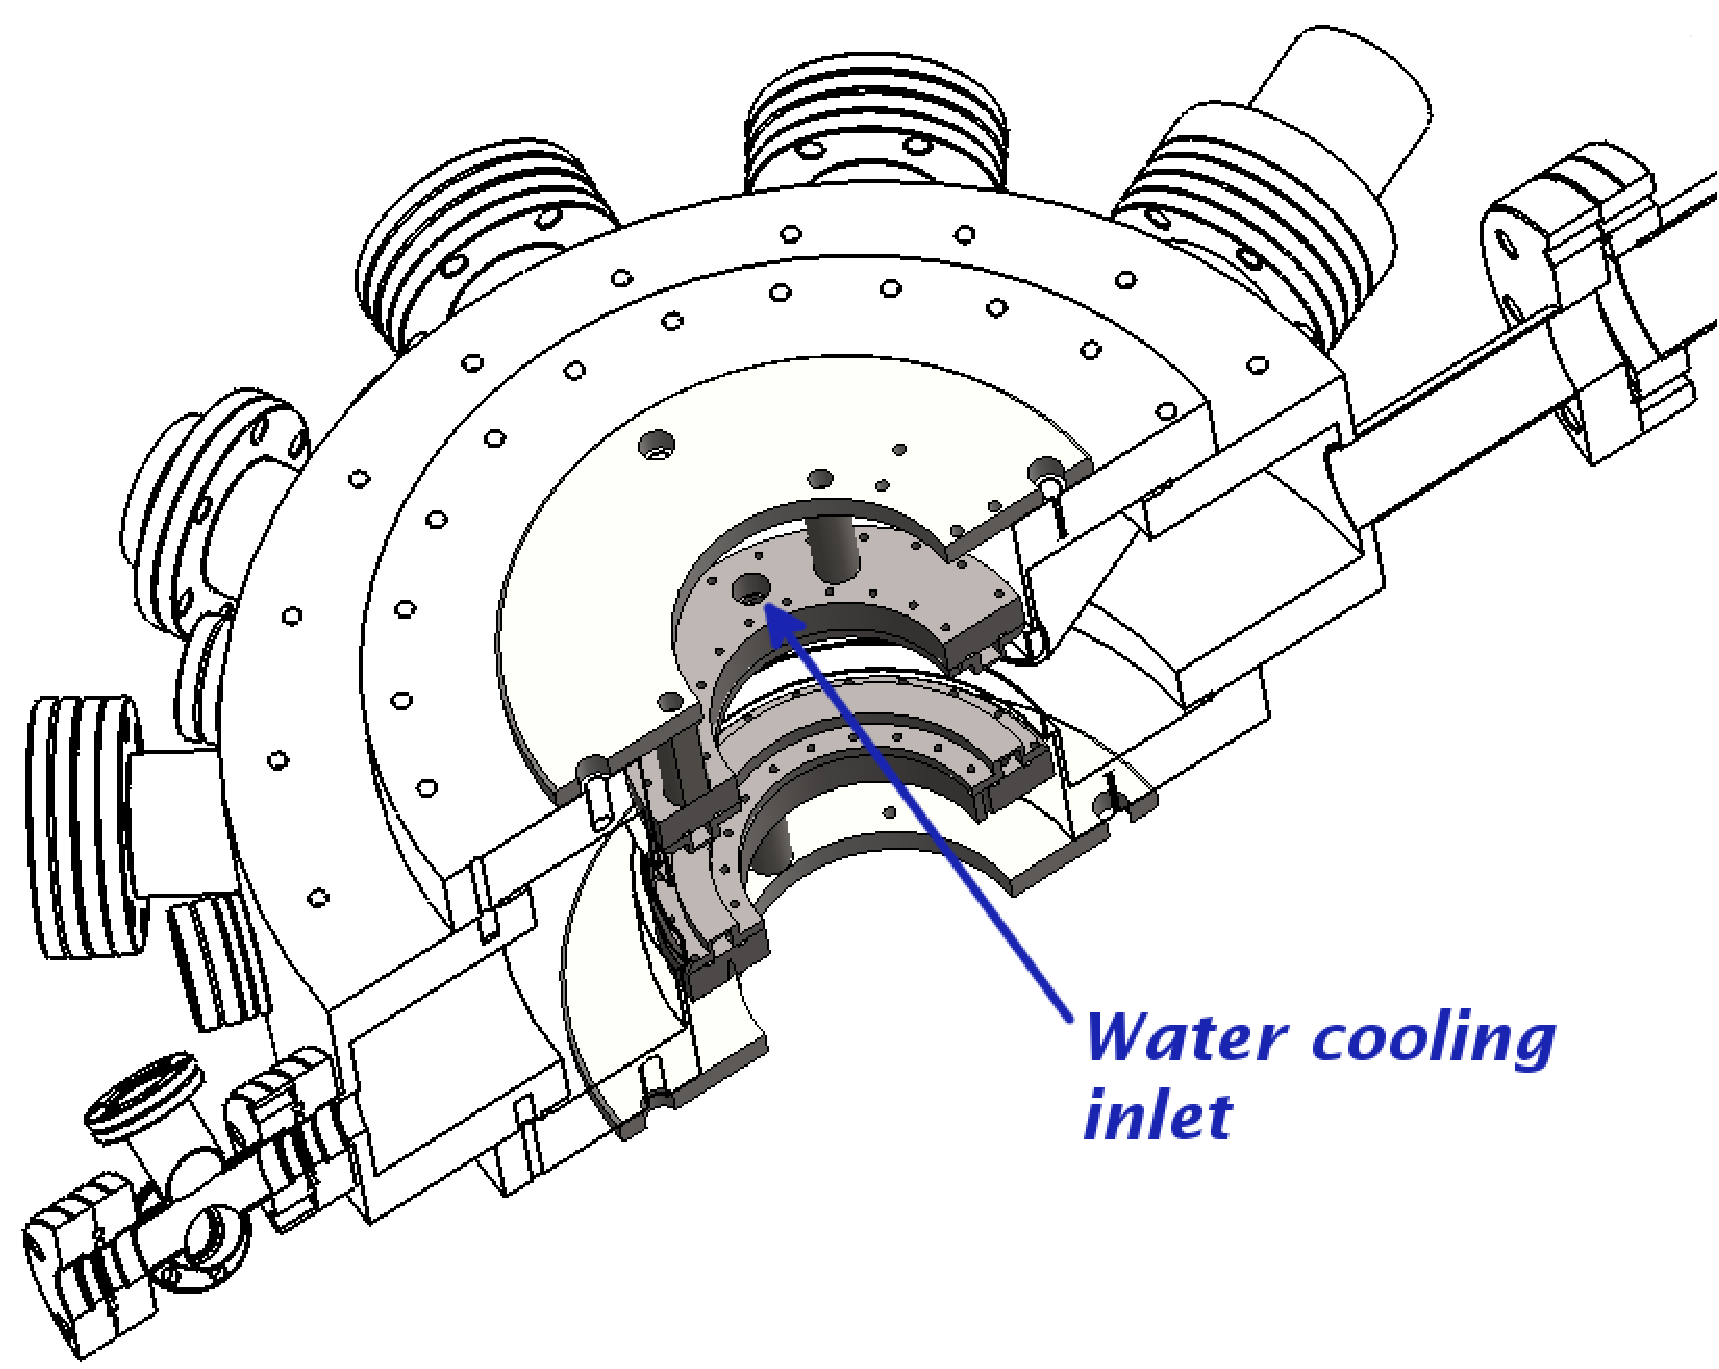
\includegraphics[width=0.45\textwidth]{../figures/coils/angleview.pdf}
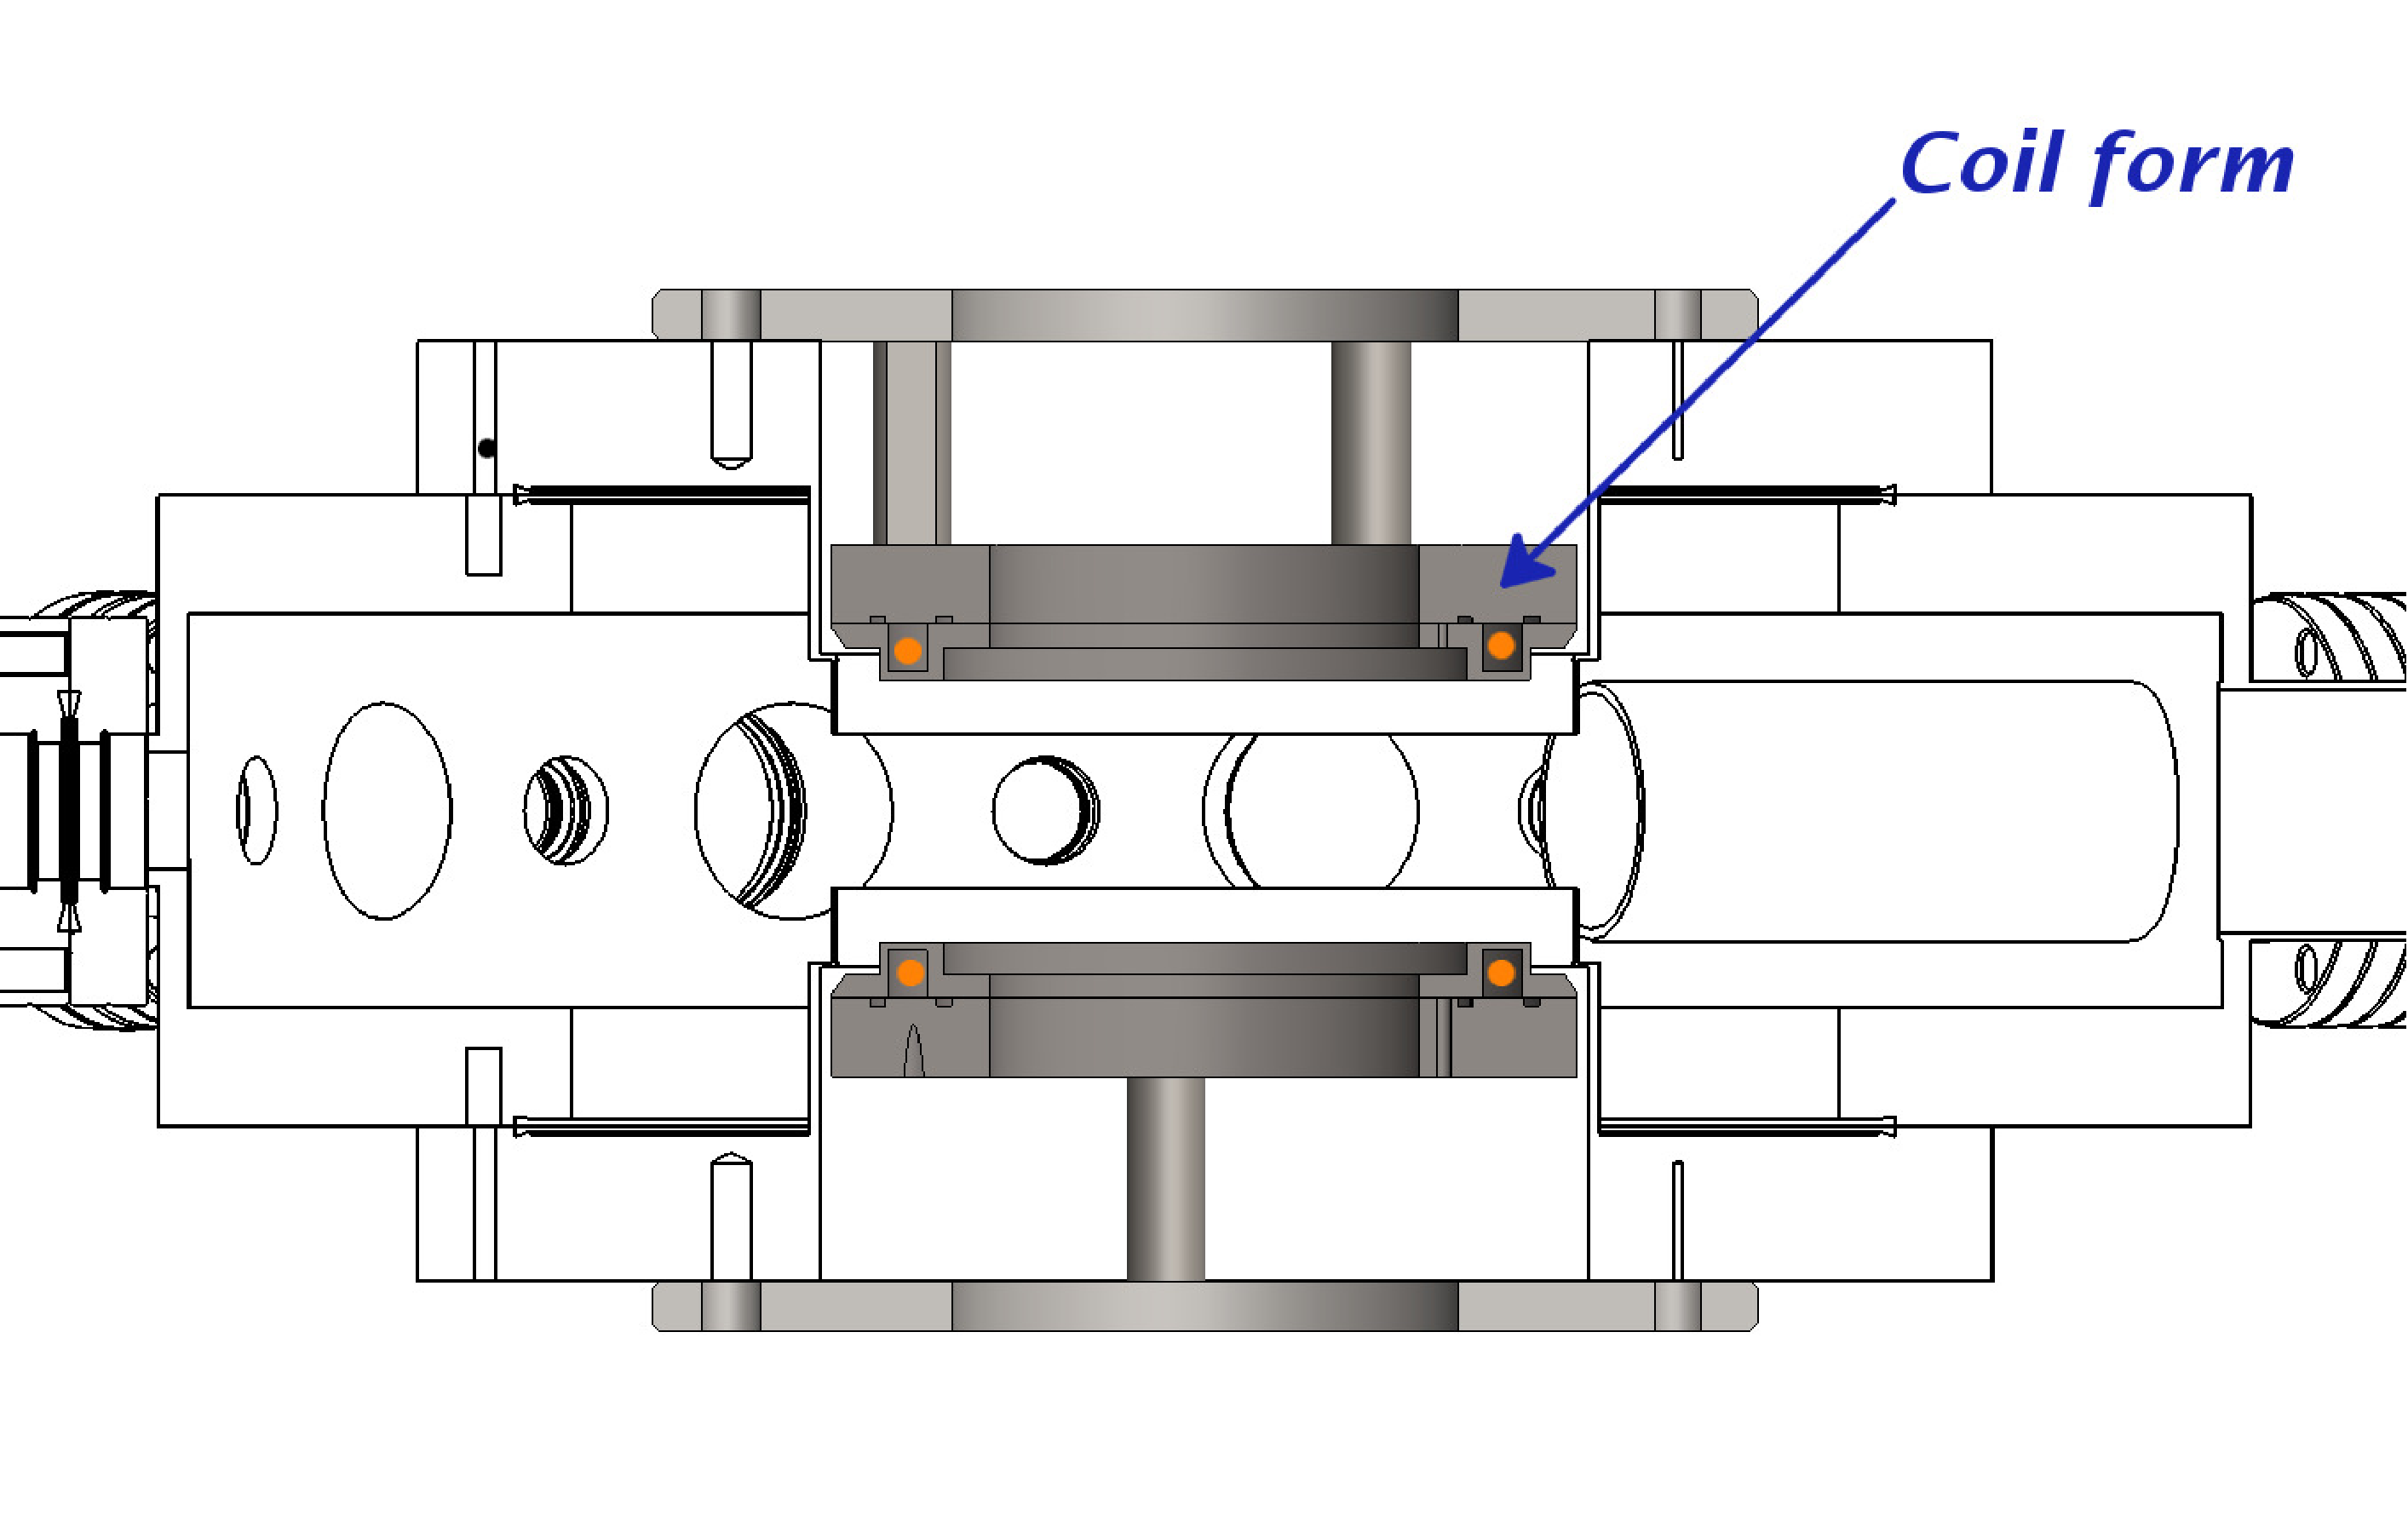
\includegraphics[width=0.55\textwidth]{../figures/coils/sideview.pdf}
\caption[Location of magnetic field coil forms ]{\small Cut-out view of our
chamber showing the location of the coils that create the magnetic field.   The
coil forms are close to the atoms inside the re-entrant top and bottom viewports.
The forms themselves are attached to a mounting plate that bolts to the
re-entrant viewport flange.  The coils are water cooled; only  the water inlet
is shown in this picture, the water outlet is on the half that is cut out. }
\label{fig:coilforms} \end{figure} The radius of the coils is 4.72~cm,
which is equal to the separation between them.  There are 35 turns on each of
the coils.  During the MOT stages of our experiment the current through the
coils is run such that they are in anti-Helmholtz configuration and produce a
magnetic field gradient along $z$, given by \[ \mathrm{d}B_{z} = \left(
\frac{4}{5} \right) ^{5/2} \frac{3}{2} \frac{\mu_{0} n I } { r^{2} } \] which
is equivalent to 1.74 G/cm/A given our configuration. 

After the optical dipole trap is loaded from the UVMOT the direction of the
current in the top coil is reversed and they produce a bias field given by \[ B
= \left( \frac{4}{5} \right) ^{3/2} \frac{\mu_{0} n I }{r}  \] which amounts to
6.8 G/A.   

%----------------------------------------
\subsection{Field control}
%----------------------------------------

The polarity of the current on the top coil is switched by using an H-bridge
made by four field-effect transistors (FETs), labeled $Q1$ to $Q4$ in
Fig.~\ref{fig:fieldcircuit}.  \begin{figure} 
\centering
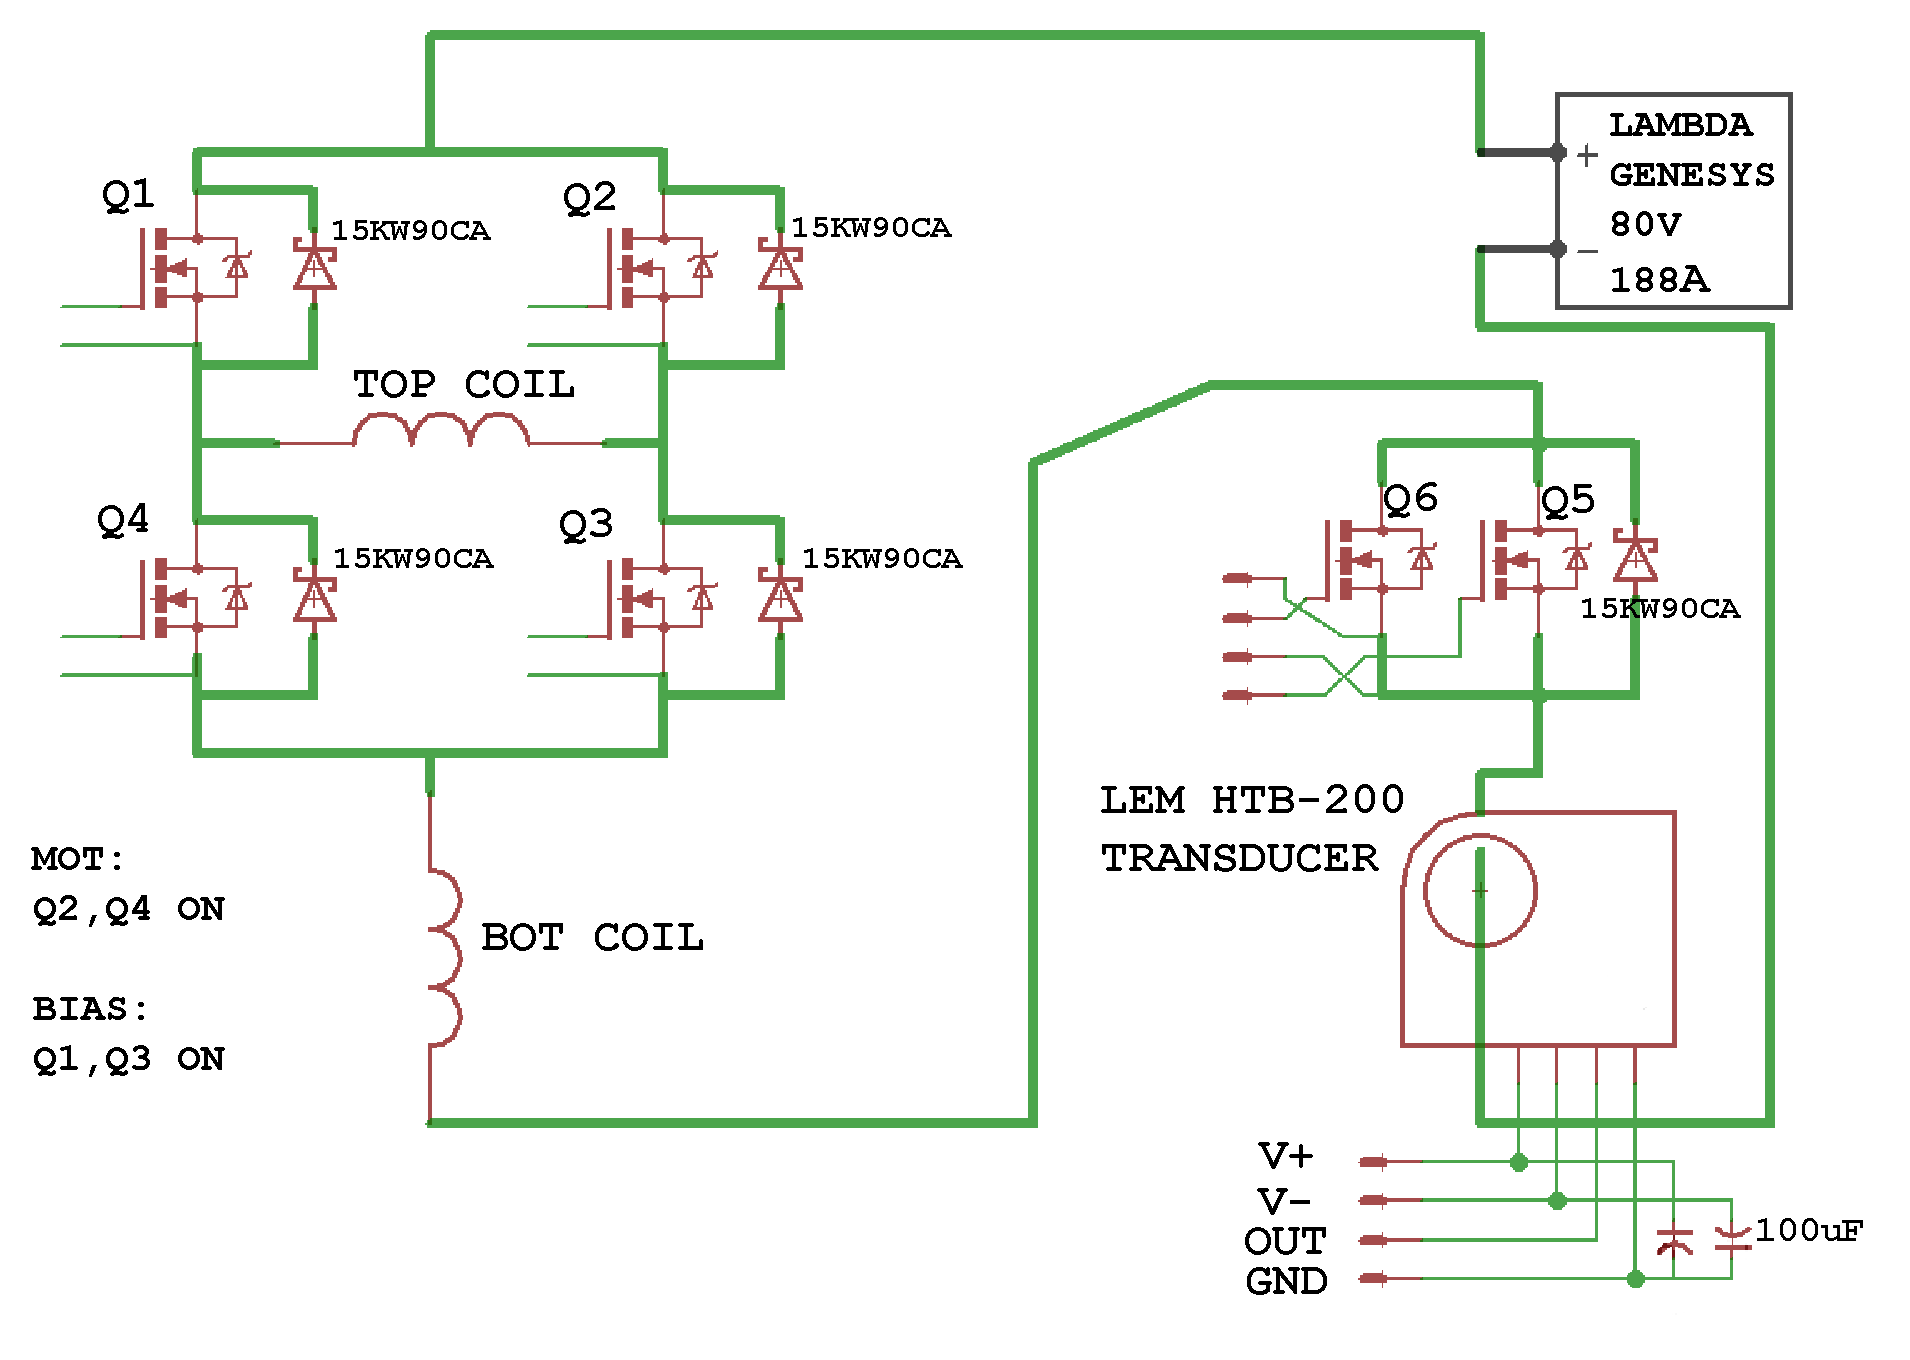
\includegraphics[width=0.85\textwidth]{../figures/coils/circuit-schematic.pdf}
\caption[Magnetic field control circuit]{\small Schematic of the magnetic field
stabilization circuit.  An H-bridge is used to reverse the polarity of the
current on the top coil.  The FET used in the H-bridge are Part Num. STE180NE10.
Two FETs in parallel, Part Num. IXFN230N10, provide active stabilization of the
current. Transient voltage suppressors, Part Num. 15KW90CA, are used across
all the FETs to reduce any voltage spikes and increase the turn-off speed of
the coils.} \label{fig:fieldcircuit} \end{figure} The current through the coils
in either gradient or bias configuration is measured with a low cost LEM
HTB-200 transducer.  The current is actively stabilized by feeding back to the
gate voltage of a pair of FET's connected in parallel, labeled $Q5$ and $Q6$ in
Fig.~\ref{fig:fieldcircuit}.  The supply, a 15~kW Lambda Genesys (80~V,
187.5~A), is operated in constant voltage mode and a value is fed forward to
its voltage control port so that the control FET's do not have to dissipate too
much power.  To perform fast magnetic field ramping we override the feed
forward circuit and set the power supply to a large enough voltage well in
advance ($\sim$100 ms) for its capacitors to charge up and let the FET's do
the fast ramping.   In this way we are able to go to from 0 to 120 A in 5 ms.
%although, performing an imaging resonance we find that it takes another 40 ms
%for the field to reach full stability at the top.
For quick turn off we have
measured it takes 100 $\mu$s to go from a current of 20 A to zero after
grounding the gate of the control FETs.  The maximum current we can achieve is
130 A which can take the field up to 884 G, past the center of the Feshbach
resonance at 834 G.   


%########################################
\section{Diagnostics}
%########################################

In order of increasing spatial resolution and sensitivity, we can detect atoms
with either a photodiode, a surveillance CCD camera, or a high performance
electron multiplying CCD camera (see Fig.~\ref{fig:diagnostics}).   We use the
photodiode to monitor the fluorescence of the atoms while they are being loaded
into the 671 nm MOT.  It is located right in front of one of the small
viewports in our chamber and a lens is used to focus the fluorescence of the
atoms onto the active area.  We use the surveillance camera to perform
diagnostics of density and temperature in the MOT via fluorescence imaging, and
the Andor EMCCD camera to take absorption images of  the atoms after they have
been loaded into  the optical dipole trap.  \begin{figure}
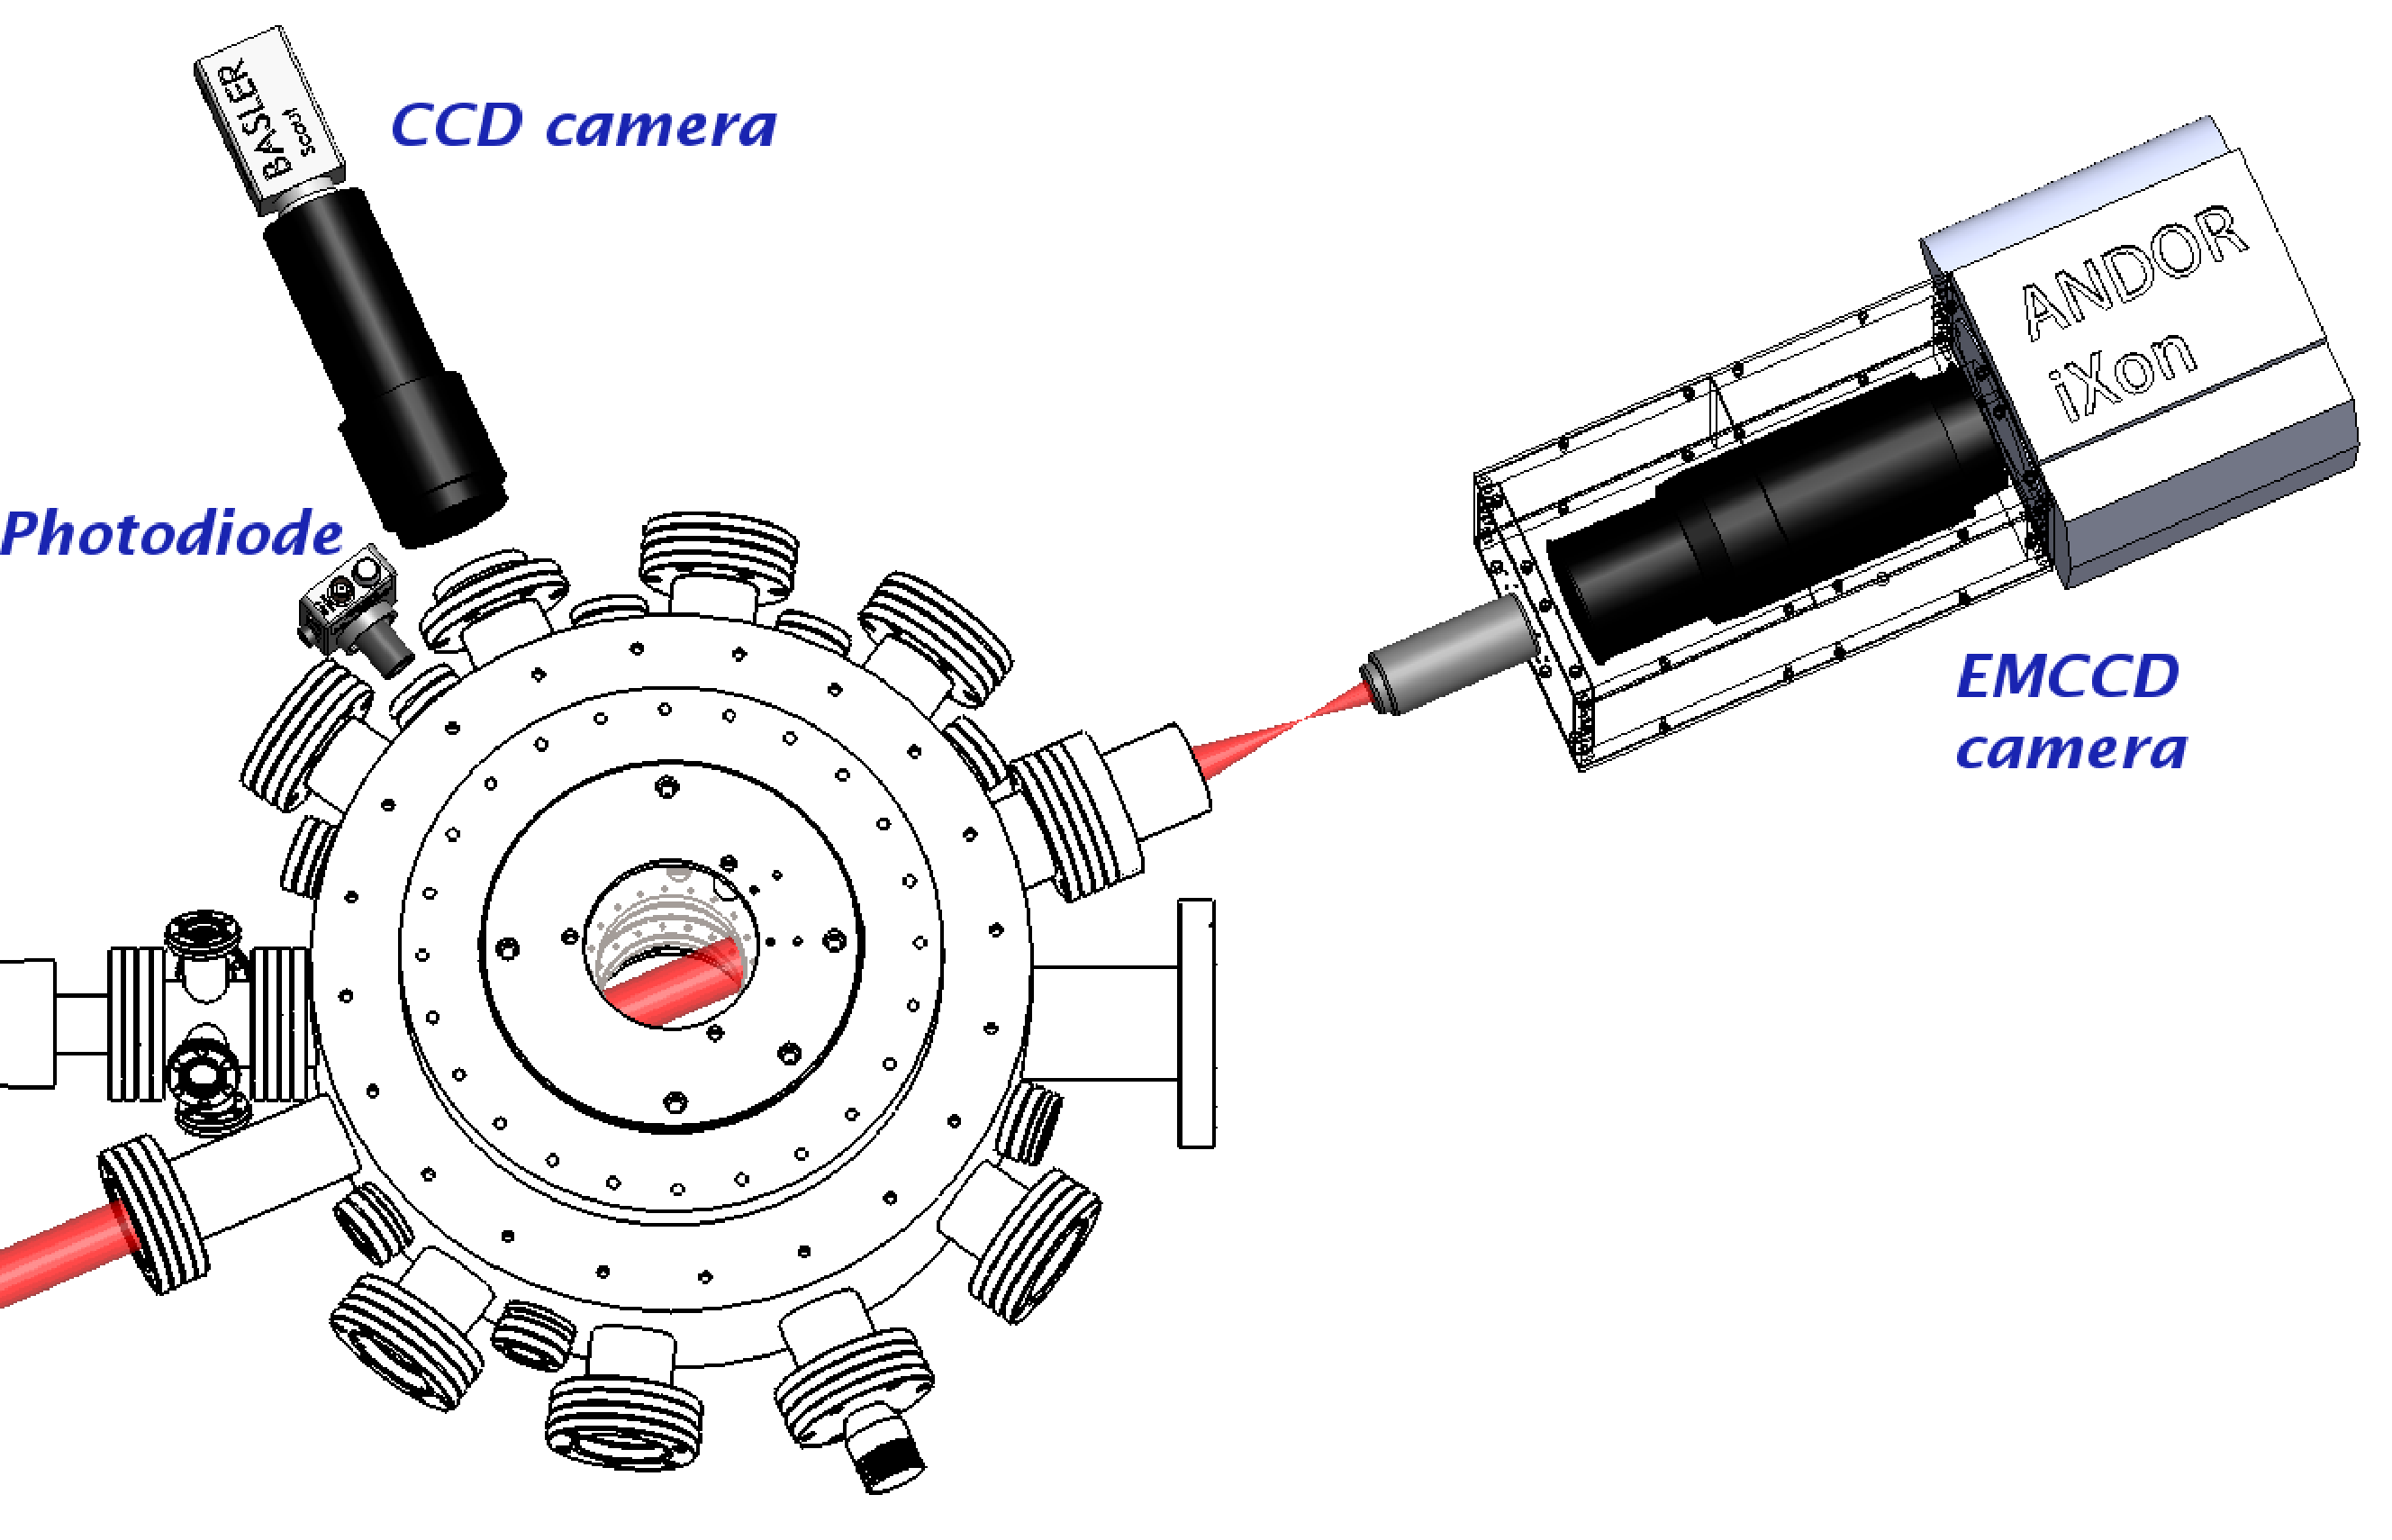
\includegraphics[width=\textwidth]{../figures/imaging/setup.pdf}
\caption[Diagnostics setup]{\small This figure shows the three instruments that
we use for atom diagnostics.  The photodiode is a DET36A from Thorlabs; a red
filter is placed in front of the photodiode to minimize the amount of ambient
light that it picks up.  We obtain a signal of about 0.75 V when the MOT is
fully loaded\footnote{Fluorescence is not necessarily indicative of number of
atoms since it can be increased for instance, by having closer detunings}.  The
surveillance CCD camera used to acquire time-of-flight images of the MOT is a
Basler scA100-30fm.  The scientific camera we use for absorption imaging is an
Andor DU-897-E.  } \label{fig:diagnostics} \end{figure} 

%----------------------------------------
\subsection{Fluorescence imaging}
%----------------------------------------

A Navitar Zoom 7000 close-focusing macro video lens is used to focus the
fluorescence from the atoms onto the CCD camera. The camera is a Basler
scA100-30fm, 1034$\times$779 pixels with 4.65$\times$4.65 $\mu$m pixel size.   To
quantitatively analyze the images taken by this camera one needs to calibrate
its collection efficiency (solid angle), its magnification and its quantum
efficiency.    

The solid angle is measured using a big iris placed at a known distance from
the atoms and then closing it up until the number of counts starts to decrease
due to the iris aperture~\cite{Junker2007}.  For the magnification and focusing
settings that we use, the solid angle was measured to be
$g=\mathrm{d}\Omega/4\pi=5.55\times10^{-3}$.  After the magnification and focus
are set, the magnification is calibrated by removing the camera from the setup
and taking a picture of a ruler placed at the distance where the atoms would be
in the actual setup.  The value is found to be $m=2.5\times10^{-3}$ cm/pixel.
The quantum efficiency is measured by taking pictures of beam with a known
power and integrating the number of counts during a certain time interval.  In
this way it is found that the efficiency of the camera is $q=13.1$ photons per
count.  We define the collection efficiency of the system as  $\epsilon= g/q$.

When taking pictures of the atoms in the MOT we first release them from the
trap by turning off the light and the magnetic field.  After a time of flight,
we pulse the MOT beams back on, typically for 100 $\mu$s,  and collect the
fluorescence on the CCD.   The population difference between the ground and
excited state of the atoms is assumed to be in steady state for the duration of
the imaging pulse\footnote{This assumption is reasonable since the exposure
time is much larger than the lifetime of the excited state}, which means that
the number of counts recorded by the CCD camera is given by \[
N_{\mathrm{counts}} = \epsilon N_{\mathrm{photons\atop scattered}} =  \epsilon
N_{\mathrm{atoms}} \rho_{ee}\frac{t_{\mathrm{exp}}}{\tau}     .\]  where
$\rho_{ee}$ is the fraction of atoms in the excited state and $\tau$ is the
lifetime of the excited state which for the \twop{3/2} state is $\tau = 27.1$
ns~\cite{McAlexander1996}.  This relationship is inverted to obtain the number
of atoms in the MOT.   

The factor $\rho_{ee}$ is hard to calculate as a function of detuning in a MOT
configuration with trapping and repumping frequencies.  However, if the beams
are on resonance, \[ \rho_{ee} =  \frac{I/\isat}{1+2I/\isat} .\] We have six
beams with 1.2\isat per beam, so on resonance $\rho_{ee}\approx 0.47$.  From
this value we can calibrate $\rho_{ee}$ as a function of detuning by changing
the detuning of the MOT lasers while taking pictures of atom clouds created
under the same conditions. 
%\footnote{ We do not use the formula \[ \rho_{ee} = \frac { I/\isat} { 1 + 4
%\frac{\Delta^{2}}{\Gamma^{2}} + 2 I/\isat}\] because it does not apply when
%one has a transition that is not cycling and two frequencies with different
%intensities. } 

It is useful to have a calibration of $\rho_{ee}$ for a large detuning because
the cloud of atoms can sometimes be so optically thick that the MOT beams are
attenuated significantly before they reach its center.  This makes the imaged
distributions look artificially flat topped.  Our preferred detuning for
imaging dense MOT clouds is $\Delta=-30$~MHz.  We have measured the calibration
factor for $\Delta=-30$~MHz and obtained \[ \rho_{ee}(
\Delta=-30\,\mathrm{MHz}) = \frac{\rho_{ee}( \Delta=0\,\mathrm{MHz})}{14.9}.\] 




%----------------------------------------
\subsection{Absorption imaging}
\label{subsec:absorption}
%----------------------------------------

Absorption imaging is performed by passing a collimated probe beam through the
atoms; the atoms scatter light from the beam and their shadow can be imaged.
In our setup the probe beam is fiber coupled to the apparatus table and then
expanded to have a $1/e^{2}$ beam waist of 2.75 mm.   A relay lens of unity
magnification (Fig.~\ref{fig:relaylens}) focuses the image of the atoms onto a
focal plane outside the vacuum system.  \begin{figure} \centering
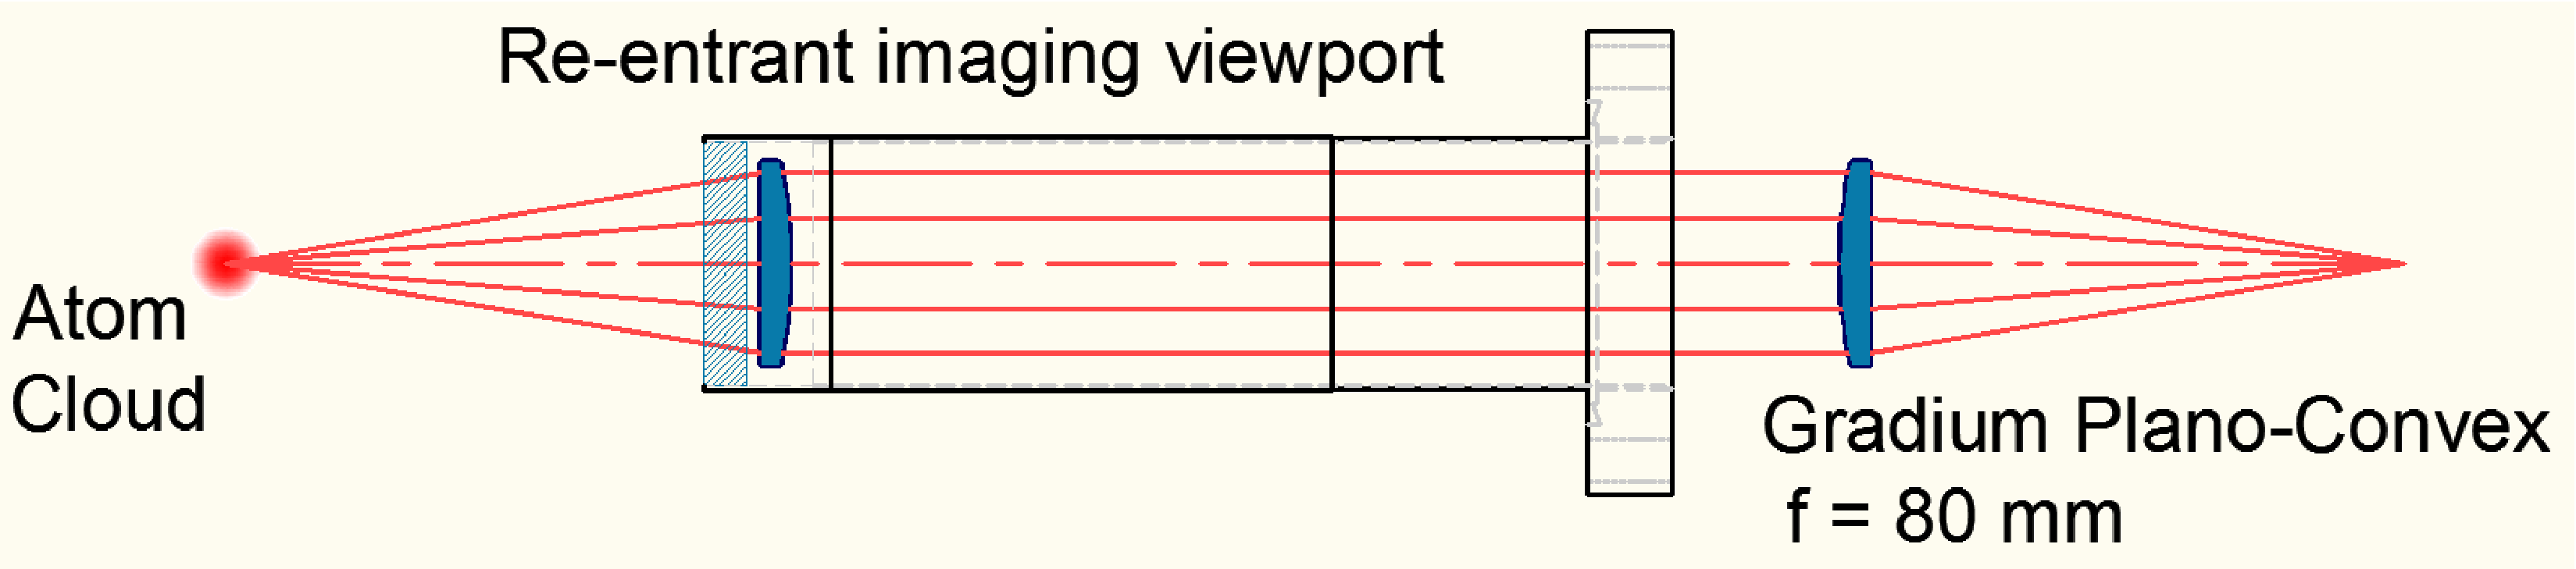
\includegraphics[width=0.85\textwidth]{../figures/imaging/relay.pdf}
\caption[Relay lens system]{\small  Relay lens system to form an image of the
atoms outside the vacuum chamber.  The lenses are gradient index plano-convex
lenses, Part Num. GPX-30-80 from LightPath Technologies. }
\label{fig:relaylens} \end{figure} The relay lens is made with  two gradient
index lenses; it is a simple setup which is robust to centration and variation
of object distance.     The numerical aperture of the relay lens system is 0.16
which gives a diffraction limited resolution of 2.6~$\mu$m using Rayleigh's
criterion.   From simulations using OSLO\footnote{Optics Software for Layout
and Optimization, Lambda Research Corporation} the relay lens with the
specified gradient index profile for the individual lenses should be
diffraction limited.  However due to the manufacturing tolerance in the index
profile we have observed this not be the case.  The resolution of the relay is
measured to be 6~$\mu$m which is not as good as than the resolution obtained by
the other experiments in our lab using a more complex five element custom made
relay lens system.

We use an infinity corrected microscope objective and a Nikon telephoto lens to
focus the relayed image on the CCD.  The Nikon telephoto lens has a variable
focal length of 70-300 mm.     For all the data taken in this thesis we used a
5x BD Plan Apo microscope objective from Mitutoyo\footnote{Infinity corrected
objectives generally specify their magnification for use with a 200 mm tube
lens. } and we set the Nikon telephoto at 200 mm to obtain a magnification of
5x. 

From an absorption image and a reference image  the column density is
obtained~\cite{Ramsey2006} as \[ \tilde{n}(x,z) = \frac{1}{3\pi\lambdabar^{2}}
\left[ ( 1+ 4\left(\frac{\Delta}{\Gamma}\right)^{2} OD(x,z) + 2
\frac{I^{\mathrm{ref}}(x,z)}{\isat} \left( 1 - e^{-OD(x,z)}\right) \right] \]
where $OD(x,z) = -\ln ( I^{\mathrm{abs}}(x,z) / I^{\mathrm{ref}}(x,z)) $.

\subsubsection{High field and low field imaging} 

It is useful to have the ability to take absorption images of the atoms  at
high magnetic field as well as low magnetic field.  At high magnetic field the
interatomic interactions can be very large due to  the wide Feshbach resonance
at 834 G.   On the other hand at low field the atoms are essentially
non-interacting.

To image at high field, the cycling transition between the $\twos{1/2}\cm
m{J}=-1/2$ state to the $\twop{3/2}\cm m_{J}=-3/2$ is used; this is the same
transition used for operation of the Zeeman slower, see
Fig.~\ref{fig:zeemanlevels}.  In our setup the probe beam propagates
perpendicular to the quantization axis defined by the magnetic field;
therefore, we can't directly drive a $\sigma^{-}$ transition.   The probe light
has a polarization perpendicular to the magnetic field and therefore equal
amounts of $\sigma^{-}$ and $\sigma^{+}$ light.  The absorption cross section
is then $3\pi\lambdabar^{2}$ instead of the maximal $6\pi\lambdabar^{2}$ and
the saturation intensity is 10.2 mw/cm$^{2}$.   


When imaging at low field one faces the problem that there is no cycling
transition.  The probe light has to have both trapping and repump frequencies
or otherwise the atoms will go into a dark state after scattering just a few
photons.   We overlap trapping and repump frequencies on a beamsplitter to
obtain the light that seeds the tapered amplifier for the 671 nm MOT.   The
beams reflected off of the beamsplitter, which also come out overlapped, are
passed through an AOM before being coupled to the imaging probe fiber.   The
low field imaging light is combined with the high field imaging light using a
polarizing beamsplitter cube.  Using a card to block one of the input sides of
the cube we can select between the low and high field imaging probes. 


%########################################
\section{Control, automation, and data analysis}
%########################################

The experiment control system in Apparatus3 is based on the National
Instruments PXI chassis NI-PXIe1062Q.   The chassis hosts a 6733 Analog Output
card and a 6259 Multifunction DAQ card.   An experimental sequence consists of
a series of TTL pulses that control the timing of events related to instruments
on the apparatus.  The clock to which TTL pulses are synchronized is an 80~MHz
oscillator on the 6259 Multifunction DAQ card.    A digital sequence can have a
maximum output rate of 10 MHz (resolution time step of 1 $\mu$s) and at this
output rate the buffer can hold sequences that last several tens of seconds.
We use the analog output channels of the PXI system as one typically uses
arbitrary waveform generators; waveform outputs can be triggered by TTL pulses
at any given time during the experimental sequence.  The timebase for arbitrary
waveform outputs on analog output channels is the on-board oscillator of each
card.  For the 6259 it is a 80 MHz oscillator and for the 6733 it is a 20MHz
oscillator.  

The experimental sequences, including all waveform outputs,  are programmed in
a format based on the Python programming language.  This makes it very easy
to program new sequences and recycle parts of old sequences.  At the moment we
have built up a library of 24 sequences  that represent the measurements that we
most commonly perform with the apparatus.   Several of these sequences are
benchmark measurements of the performance of every stage of the experiment that
we run every day before picking up where we left the day before.   

The Python  based sequence code is interpreted by a program written also in
Python which produces a raw sequence output file that contains all the TTL
timings and the waveforms for a particular experiment.  The raw sequence output
is read by LabVIEW, which takes care of outputting the sequence on the TTL and
analog output channels.  For most of our experiments $t=0$ is the moment when
the MOT has loaded to a desired fluorescence, as measured by the monitoring
photodiode.   When the fluorescence reaches the desired level, the output of
the experimental sequence is triggered.

Our scheme for taking, saving and analyzing data is based around the ubiquitous
concept of the report file; it is explained in Fig.~\ref{fig:daq}. 
\begin{figure}
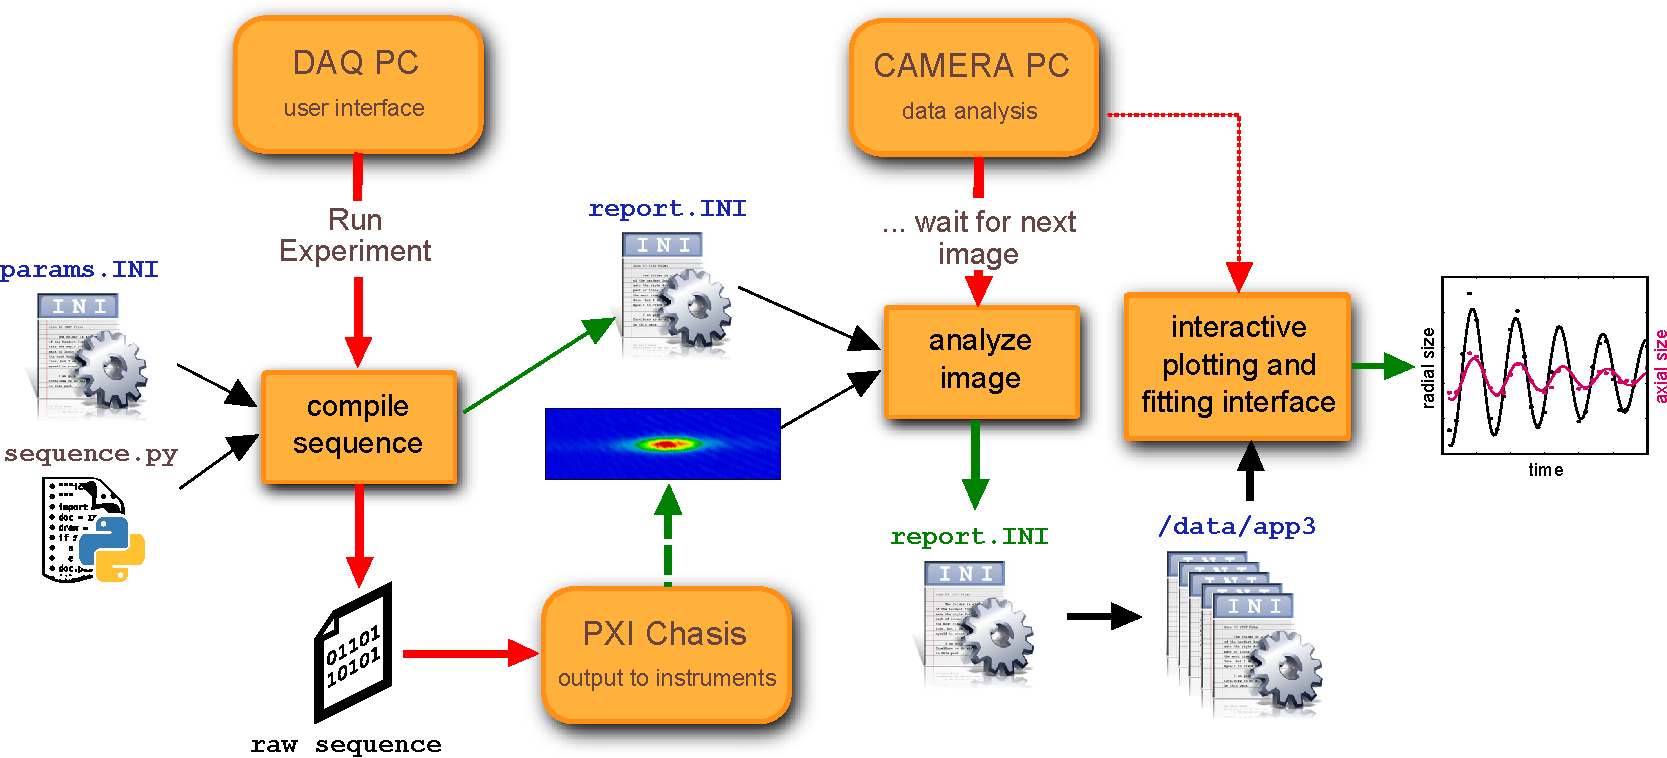
\includegraphics[width=\textwidth]{../figures/control/daq-schematic.pdf}
\caption[Data acquisition flowchart]{\small  This figure attempts to show the
flow of information during one experimental run.  The hardware is represented
by the rounded rectangles and the processes running on the hardware are
represented by the straight rectangles.  The red lines represent flow, the
black lines represent input to a process and the green lines represent the
output of a process. \par  When an experiment is run, the raw sequence is
compiled based on the sequence file and params.INI.   A report file is created
at this time.  The image of the atoms is analyzed by the camera computer and
results of the analysis are stored inside report.INI which also contains all
the parameters relevant for a given image.   The plotting and fitting interface
queries information from the reports on disk and produces graphs of the
measured phenomena.  The plot shown is the result of the measurement of the
frequency of the radial breathing mode for our optical dipole trap. }
\label{fig:daq} \end{figure} All the parameters for all the experimental
sequences in our library are stored in a file called \verb$params.INI$ that the
user can edit using a regular text editor.   Values are separated in sections
following the INI file convention, making it easy to scroll through the 200
long and growing parameter list.   When a user runs an experiment, the sequence
is compiled according to the sequence description given in the Python format
file, where variables take the values indicated by \verb$params.INI$.  \,During
compilation a copy of \verb$params.INI$ is created called \verb$report.INI$.
This report will be from then on associated with this particular shot. LabVIEW
reads the compiled raw output sequence and runs the experiment; the camera
computer acquires the images from the Andor camera and saves them to disk.
Using information about the shot, contained in \verb$report.INI$, the image of
the atoms is analyzed and any results of the analysis, such as atom number,
density, cloud size, temperature, etc., are stored in a new section inside the
same report file.   The report file thus contains all information relevant to a
shot and the results of its analysis.  An interactive plotting and fitting
graphical user interface queries the report files in the data directory and
allows us to see the processed data as it comes out in real time.   The report
file concept makes it particularly easy to revisit old data. 

Analysis of the images is done in real time and as we take pictures at a rate
of about 1 every 10 seconds it was necessary to write the code in C++ to avoid
the analysis from hanging back.  Our code is benchmarked to fit a reasonable
looking cloud of atoms to a 2D-Gaussian distribution on a 512x512 pixel grid
within 8-12 seconds. 1D-Gaussian fits on a row of 512 pixels take less than
half a second.   The graphical user interface which plots and fits data is
written in Python. 




%%%%%%%%%%%%%%%%%%%%%%%%%%%%%%%%%%%%%%%%%
%%%%%%%%%%%%%%%%%%%%%%%%%%%%%%%%%%%%%%%%% 
\chapter[Narrow linewidth $^{6}$Li magneto-optical trap]{Narrow linewidth
$^{6}$Li magneto-optical trap\footnote{In this chapter I use
$\isat^{2P}=5.1\,\mathrm{mW/cm^{2}}$ for the saturation intensity of the 671~nm
transition and $\isat^{3P}=5.9\,\mathrm{mW/cm^{2}}$ for the saturation
intensity of the 323~nm transition.  Recall $\isat= \frac{2\pi h
c\Gamma}{3\lambda^{3}}$.}} \label{ch:uvmot}
%%%%%%%%%%%%%%%%%%%%%%%%%%%%%%%%%%%%%%%%%
%%%%%%%%%%%%%%%%%%%%%%%%%%%%%%%%%%%%%%%%% 

The UVMOT  cools \li atoms to a temperature of 57 $\mu$K by cycling photons on
the narrow \uv transition.   In this chapter I describe the procedure to load
the UVMOT and show the results of its characterization.  
%I first give details
%about the 671 nm MOT and then explain how we transfer the atoms to the UVMOT.

%########################################
\section{671 nm MOT}
%########################################
The 671 nm MOT is loaded from a Zeeman slower plus a 2DMOT. The 2DMOT is at the
output of the Zeeman slower and helps collimate the slow thermal beam of atoms
before it reaches the MOT.  In 5~s we load 1.4$\times10^{9}$ atoms in the
MOT at a temperature of $\approx$780~$\mu$K.  After loading to the desired fluorescence
level we shutter the Zeeman slower laser using a hard disk drive
shutter~\cite{HardDriveShutter2007}.   At this point we
proceed to cool and compress the 671 nm MOT by  reducing the intensity and
detuning of the the cooling and repumping light, and increasing the magnetic
field gradient to the values shown as CMOT on Table.~\ref{tab:cmot}.
\begin{table}

\centering
\scalebox{1.0}{
\begin{tabular}{l|cc|c}
 &  MOT & CMOT & unit\\
\hline  \hline \noalign{\smallskip}
Trap intensity per beam   & 1.26 & 0.034 & $\isat^{2P}$ \\
Trap detuning   & -33 & -12 & MHz\\
Repump intensity per beam & 0.36 & 0.007 & $\isat^{2P}$ \\
Repump detuning & -25.2 & -17 & MHz\\
$dB_{z}$  & 22.6 & 26.1  & G/cm \\ 
\hline \noalign{\smallskip}
Number & 1.5  & 1 & $10^{9}$\\
$1/e$ radius & 0.22 & 0.18  & cm\\
Peak density  & 2.39 & 3.40 & $10^{10}$cm$^{-3}$\\ 
Temperature & 783 & 288 & $\mu$K\\
Phase space density &  3.9$\times 10^{-7}$ & 2.5$\times 10^{-6}$ & -  
\end{tabular}}
\caption[671 nm MOT cooling and compression]{\small Comparison between the
settings used for loading the 671 nm MOT and the settings after cooling and
compressing (CMOT).   For cooling and compressing, first the field gradient is
increased in 40 ms, then after a wait of 40 ms the intensity and detuning of the
beams are ramped linearly to their final values in 1 ms.   The phase space
density is defined as $n_{0}\lambda_{T}^{3}$ where $n_{0}$ is the peak density
 and $\lambda_{T}=\frac{h}{(2\pi m \kb T)^{1/2}}$  is the thermal de Broglie 
wavelength. } 
\label{tab:cmot}
\end{table}
 We take time-of-flight images of
the MOT and the CMOT, and infer their temperatures by fitting the cloud sizes
to a ballistic expansion as shown in Fig.~\ref{fig:cmotexp}.   
\begin{figure} \hspace{0.16\textwidth}
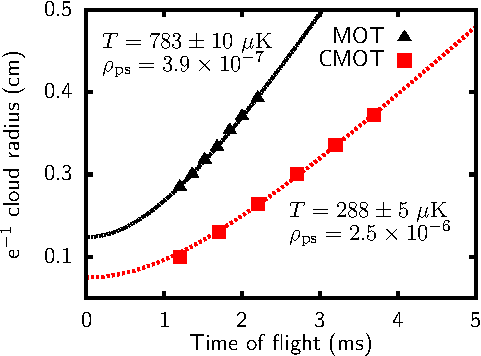
\includegraphics[width=0.58\textwidth]{../figures/323mot/tofexpansion-00/tofeps-SS.pdf}
\caption[671 nm cooled and compressed MOT]{\small  Time-of-flight expansion of
atoms released from the 671 nm MOT right after loading (black triangles) and after
cooling and compressing (red squares). The points represent the $1/e$ width of
Gaussian fits to the spatial profile of the freely expanding clouds.  The lines
are fits to ballistic expansions. } \label{fig:cmotexp} \end{figure}
 
%########################################
\section[323 nm MOT]{323 nm MOT}
%########################################

The first implementation of the UVMOT used repump light on the red transition
instead of the UV transition.  We later implemented a repump on the UV
transition and found that the number of atoms loaded into the UVMOT increased
by a factor of 2 and the density increased by a factor of 1.5 while the
temperature stayed the same.   This numbers also translated into better
efficiency in loading the optical dipole trap. 

%----------------------------------------
\subsubsection{UVMOT with red repump}
%----------------------------------------


The UVMOT 
 is loaded from the CMOT as shown in the timing diagram in Fig.~\ref{fig:timing}.
\begin{figure} \centering
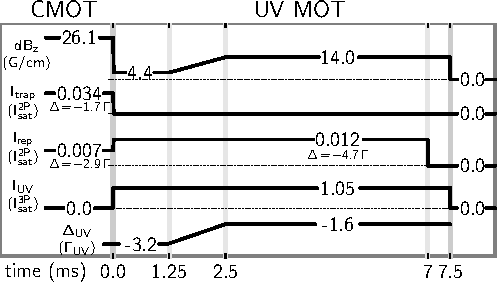
\includegraphics[width=0.5\textwidth]{../figures/323mot/timingdiagram-00/timing.pdf}
\caption[UVMOT loading timing diagram]{\small Timing diagram representing the
transfer sequence from the CMOT to the UVMOT using a red repumper. } \label{fig:timing} \end{figure}
Loading occurs by abruptly reducing the magnetic field gradient, turning off
the red cooling light, and turning on the UV cooling light.  The loading phase
lasts for 1.25 ms and consists of having a small magnetic field gradient to
capture high velocity atoms from the red MOT.   The reduction of the magnetic
field gradient is critical given the narrower linewidth of the \uv transition.
After the  loading phase, we linearly increase the magnetic gradient and reduce
the detuning of the UV cooling light over 1.25 ms.  The values of this steady
state UVMOT are chosen to optimize loading to an optical dipole trap as will be
described in Chapter~\ref{ch:alloptical}.  After a hold time of 5 ms the atoms
are released and subsequently imaged with the Basler camera. A comparison of
the performance of the CMOT and UVMOT is shown in
Fig~\ref{fig:uvtexp}.  Table~\ref{tab:uvmot} shows the settings and results for the UVMOT.
\begin{figure} \hspace{0.16\textwidth}
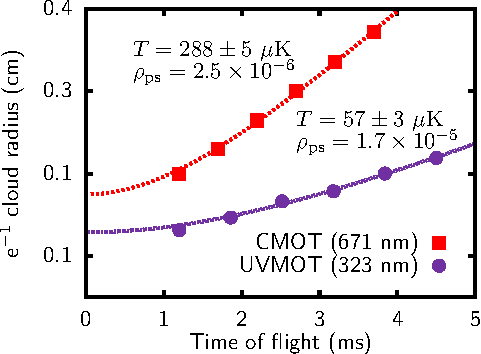
\includegraphics[width=0.58\textwidth]{../figures/323mot/tofexpansion-00/tofeps.pdf}
\caption[CMOT and UVMOT with red repump time-of-flight expansion]{\small Time-of-flight
expansion of the CMOT (red squares) and the UVMOT with red repump (violet circles).   The
points represent the $1/e$ width of Gaussian fits to the spatial profile of the
freely expanding clouds.  The lines are fit to ballistic expansions. }
\label{fig:uvtexp} \end{figure} 
\begin{table} \centering 
\scalebox{1.0}{
\begin{tabular}{l|c|c} 
&  UVMOT  & unit\\ 
\hline  \hline \noalign{\smallskip} 
Repump intensity per beam & 0.012 & $\isat^{2P}$\\ 
Repump detuning (MHz) & -27.6 & MHz \\ 
$dB_{z}$ Final & 14 & G/cm \\ 
\hline \noalign{\smallskip}
SHG Output power &  25 & mW \\
UV intensity per beam & 0.96 & $\isat^{3P}$ \\
UV detuning final & -1.6 & MHz \\
\hline \noalign{\smallskip} 
Number & 2.4 & $10^{8}$  \\ 
$1/e$ radius & 0.13  & cm \\ 
Peak density & 2.0  & $10^{10}$\,cm$^{-3}$ \\ 
Temperature & 57 & $\mu$K \\ 
Phase space density &  1.7$\times 10^{-5}$ & - 
\end{tabular}}
\caption[UVMOT with red repump settings]{\small Settings and results for the
UVMOT with red repump.} \label{tab:uvmot} \end{table} 

Repumping on the
red transition effectively reduces the narrow line character of the UVMOT.
Despite this, we still achieve $T\ll\TD=140$~$\mu$K, most likely owing to the
strength of  cooling on the UV transition compared to heating on the red.  The
amount of power on the red repumping frequency that we use corresponds to only
0.012~$\isat^{2P}$, obtained with 7~mW of injection to the tapered amplifier.
We observe that using less  power on the red repump does not affect the
performance of the UVMOT as shown in Fig.~\ref{fig:uvrep}.  
\begin{figure}
\centering
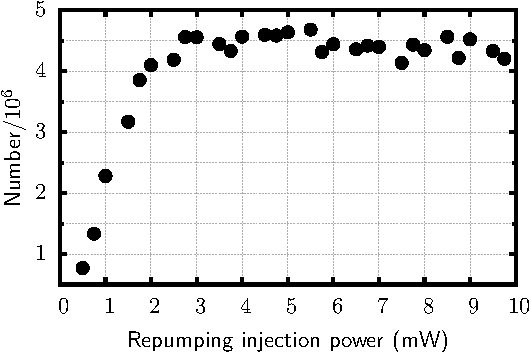
\includegraphics[width=0.55\textwidth]{../figures/323mot/uvreppow/uvreppoweps.pdf}
\caption[UVMOT performance vs. red repump power]{\small Number of atoms loaded into
optical dipole trap versus injection power of red repump into the tapered amplifier.  
The performance of the UVMOT is not affected until the injection power goes below
3~mW.   The intensity required on the red repump is only about $\isat^{2P}/100$
whereas the intensity used on the UV light is around $\isat^{3P}$.  }
\label{fig:uvrep} \end{figure}

%----------------------------------------
\subsubsection{UVMOT with UV repump}
%----------------------------------------

The timing diagram for loading the UVMOT with UV repump from the CMOT is shown
in Fig.~\ref{fig:timingUV}.  The expansion plots and values for the parameters
and results are in Fig.~\ref{fig:uvtexpUV} and Table.~\ref{tab:uvmotUV}
respectively. 

\begin{figure} \centering
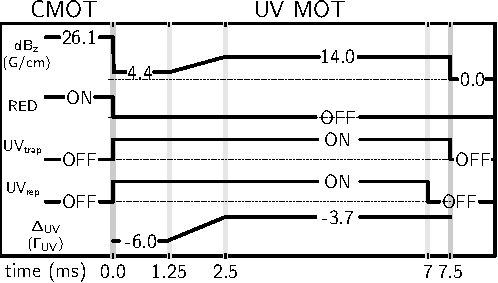
\includegraphics[width=0.5\textwidth]{../figures/323mot/timingdiagram/timing.pdf}
\caption[UVMOT loading timing diagram]{\small Timing diagram representing the
transfer sequence from the CMOT to the UVMOT. } \label{fig:timingUV} \end{figure}

\begin{figure}
\hspace{0.16\textwidth}
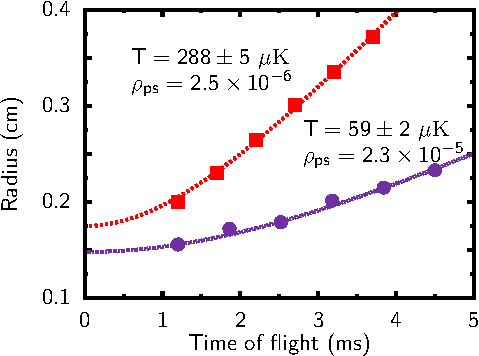
\includegraphics[width=0.58\textwidth]{../figures/323mot/tofexpansion/tofeps.pdf}
\caption[CMOT and UVMOT time-of-flight expansion]{\small Time-of-flight
expansion of the CMOT (red squares) and the UVMOT with UV repump (violet circles).  
The points represent the $1/e$ width of Gaussian fits to the spatial profile of the
freely expanding clouds.  The lines are fit to ballistic expansions. }
\label{fig:uvtexpUV} \end{figure} 

\begin{table} \centering 
\scalebox{1.0}{
\begin{tabular}{l|c|c} 
&  UVMOT  & unit\\ 
\hline  \hline \noalign{\smallskip} 
$dB_{z}$ Final & 14 & G/cm \\ 
\hline \noalign{\smallskip}
SHG Output power &  25 & mW \\
UV trap intensity per beam & 1.0 & $\isat^{3P}$ \\
UV repump intensity per beam & 0.1 & $\isat^{3P}$ \\
UV detuning final & -1.6 & MHz \\
\hline \noalign{\smallskip} 
Number & 5.3 & $10^{8}$  \\ 
$1/e$ radius & 0.15  & cm \\ 
Peak density & 2.9  & $10^{10}$\,cm$^{-3}$ \\ 
Temperature & 59 & $\mu$K \\ 
Phase space density &  2.3$\times 10^{-5}$ & - 
\end{tabular}}
\caption[UVMOT settings]{\small Settings and results for the UVMOT with UV repump.} \label{tab:uvmotUV} \end{table}
 
%----------------------------------------
\subsubsection{Effect of 323 nm power on the UVMOT}
%--------------------------	--------------

Typically 5$\times 10^{8}$ atoms are captured in the UVMOT, corresponding to an
efficiency of 50\%.  The loss of atoms is most likely due to small UV beam
waists, which are smaller than the size of the atom distribution in the CMOT.
The waists are limited by the total available power at 323 nm.  The effect of
the available power was studied by looking at the number of atoms loaded into
the optical dipole trap as a function of UVMOT intensity.  The results are
shown in Fig.~\ref{fig:uvpow}.  \begin{figure} \centering
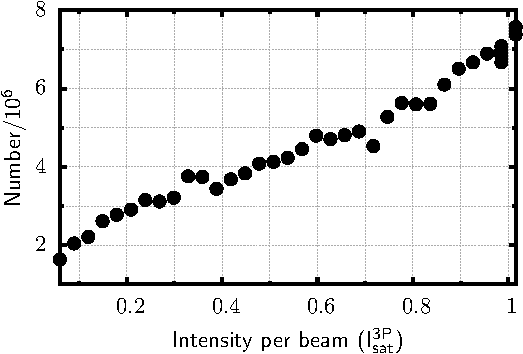
\includegraphics[width=0.55\textwidth]{../figures/323mot/uvpower/uvpoweps.pdf}
\caption[UVMOT performance vs. power]{\small Atoms loaded into optical dipole
trap (see Chapter~\ref{ch:alloptical}) as a function of UVMOT intensity per
beam.  The output power of the SHG when this curve was taken was 26.7~mW, which
gives a maximum of 1.05~$\isat^{3P}$ per beam.} \label{fig:uvpow} \end{figure} 

%----------------------------------------
\subsubsection{Effect of detuning on the UVMOT}
%----------------------------------------

The effect of detuning of the 323~nm light on the performance of the UVMOT is
shown in Fig.~\ref{fig:uvdet}.   
\begin{figure}
\centering
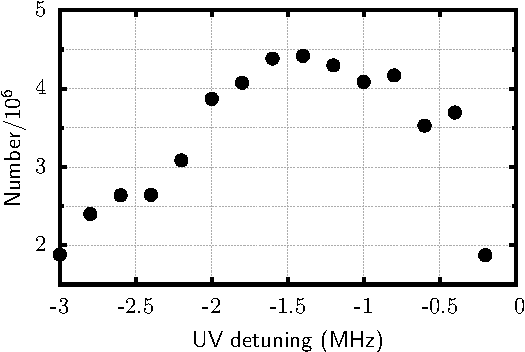
\includegraphics[width=0.55\textwidth]{../figures/323mot/uvdet/uvdeteps.pdf}
\caption[UVMOT performance vs. detuning]{\small Number of atoms loaded into
optical dipole trap versus UV light detuning. }
\label{fig:uvdet} \end{figure} 


%----------------------------------------
\subsubsection{Photoionization}
%----------------------------------------

The presence of UV light presents two-photon pathways to photoionize the atom.
An atom excited by the red laser to the \twop{3/2} state can be photoionized by
a UV photon, or an atom excited to the \trep{3/2} state by a UV photon can be
photoionoized by scattering a red photon.  For the case of the UVMOT with red
repump we have investigated both of these processes by shining far detuned UV
light on the red MOT (Fig.~\ref{fig:photoion}) or far detuned red light on the
UVMOT and we do not see a reduced lifetime in either of these situations.  An
atom in the \trep{3/2} state could also be photoionized by scattering a UV
photon.  This process, however, has a significantly smaller cross section since
it leaves the electron far higher in the continuum~\cite{Nadeem2011}.
\begin{figure} \centering
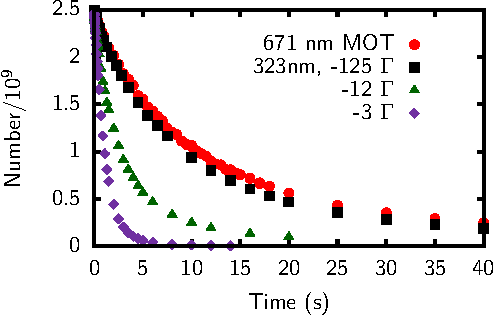
\includegraphics[width=0.55\textwidth]{../figures/323mot/photoionization/phioneps.pdf}
\caption[Photoionization with UV light]{\small Atoms remaining in steady state
red MOT as a function of time.  The lifetime of the MOT is affected when UV
light that is close to resonance is shined on the atoms (purple diamonds).  For
atoms away from the center, the UV light is blue detuned due to the magnetic
field gradient of the red MOT, $dB_{z}=22.6$~G/cm, and causes a faster loss of
atoms from the trap.  Far off-resonance light has a much smaller effect on the
MOT lifetime (red circles), putting an upper limit on photoionization rate.
The estimated photoionization rate, for a worst case scenario cross section of
2$\times 10^{-17}$~cm$^{2}$~\cite{Nadeem2011}, is less than 1 event per second.
} \label{fig:photoion} \end{figure}



%%%%%%%%%%%%%%%%%%%%%%%%%%%%%%%%%%%%%%%%%
%%%%%%%%%%%%%%%%%%%%%%%%%%%%%%%%%%%%%%%%% 
\chapter{All-optical production of a degenerate Fermi gas} 
\label{ch:alloptical}
%%%%%%%%%%%%%%%%%%%%%%%%%%%%%%%%%%%%%%%%%
%%%%%%%%%%%%%%%%%%%%%%%%%%%%%%%%%%%%%%%%% 


%########################################
\section{Evaporation near a Feshbach resonance}
%########################################

After we have cooled the atoms in the UVMOT we load them into the optical
dipole trap by quickly turning on the light power in the trap when we have
reached the steady state values of the UVMOT, at 2.5~ms in the timing diagram
shown in Fig.~\ref{fig:timing}.  We find that laser cooling on the UV
transition is effective in the trap (more on this on Sec.~\ref{sec:lightshift})
so we leave the UV and red repumping light on for the 5~ms following turning on
the optical trap.  During the last 0.5~ms of loading the red repumper is turned
off to optically pump the atoms to the \f{1/2}\cm$\mf{\pm1/2}$ states ( \one
and \two  in Fig.~\ref{fig:zeemanlevels}).  Next the UV light and magnetic field
gradient are abruptly switched off. 

Our experimental procedure continues by inverting the polarity of the top coil,
and then energizing the coils to produce a bias magnetic field.   In 20~ms we
go to 330~G, where the scattering length is $\sim -280a_{0}$.  We perform
evaporative cooling at 330~G instead of near the Feshbach resonance at 834~G
because we observe density dependent loss in the unitary scattering regime that
is fast enough to reduce the efficiency of evaporation~\cite{Du2009}.  This
loss is unobservable at 330~G.  At 280 $a_{0}$ and for a sample at 70~$\mu$K
$ka \approx 1$  and the collision cross section is nearly unitarity limited
which leads to efficient evaporation due to the high collision rates of the
order of 10$^{5}$ per second~\cite{Gehm2003}. 


We leave the trap depth at its maximum value for 200~ms and after unforced
evaporation we obtain 6$\times 10^{6}$ atoms at a temperature of 60~$\mu$K,
corresponding to $T/\TF \approx 2.7$, where $\TF= \hbar
(\omega_{\mathrm{r}}^{2} \omega_{\mathrm{a}} 3N)^{1/3}$.  After 6~s of forced
evaporation following the evaporation trajectory shown in Fig.~\ref{fig:evap},
a degenerate sample is obtained with 3$\times 10^{6}$ atoms at $T/\TF = 0.45$. 

\begin{figure} \centering
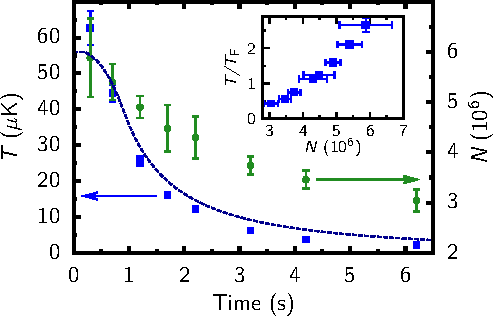
\includegraphics[width=0.75\textwidth]{../figures/evaporation-simple-01/evapeps.pdf}
\caption[Forced evaporation to quantum degeneracy]{\small Number $N$ (green
circles) and temperature $T$ (blue squares) of atoms in the optical trap during
forced evaporation. Error bars for $N$ are one standard deviation of the mean
value of $N$ for a sample of 5 measurements.  The dotted blue line is the trap
depth  divided by a factor of 5, indicating the evaporation trajectory. The
inset shows $T/T_F$ for the points in the main plot.  For $T/T_F<1$ a surface
fit to a polylog~\cite{Butts1997, DeMarco2001, Making2007} was used to determine $T/T_F$;
otherwise, $T$ was measured by ballistic expansion and $T_F$ obtained from the
mean value of $N$ and the measured trap frequencies.  Systematic uncertainties
in all measured quantities are estimated to be 10\%.} \label{fig:evap}
\end{figure} 

%########################################
\section{Light shift measurement for our optical trap}
\label{sec:lightshift}
%########################################

Intrinsic to the capability of the UVMOT to load atoms into the dipole trap is
the ability to continue to laser cool on the UV transition in the presence of
the light field of the optical trap.   Cooling in the optical trap only works
if the AC Stark shift of the cooling transition for the wavelength of the trap
light is on the order of the linewidth of the transition.  It is best when the
AC Stark shift vanishes altogether, which defines the magic wavelength for the
transition~\cite{Katori2003}. 

Our dipole trap operates at 1070~nm, close to the expected magic wavelength for
the \uv transition.  The polarizabilities of the $2S$, $2P$, and $3P$ states
have been calculated by Marianna Safronova. Her results, reproduced in
Fig.~\ref{fig:safronova}, show that there is a steep dependence on wavelength
of the polarizability of the $3P$ state near 1070~nm.  \begin{figure}
\centering 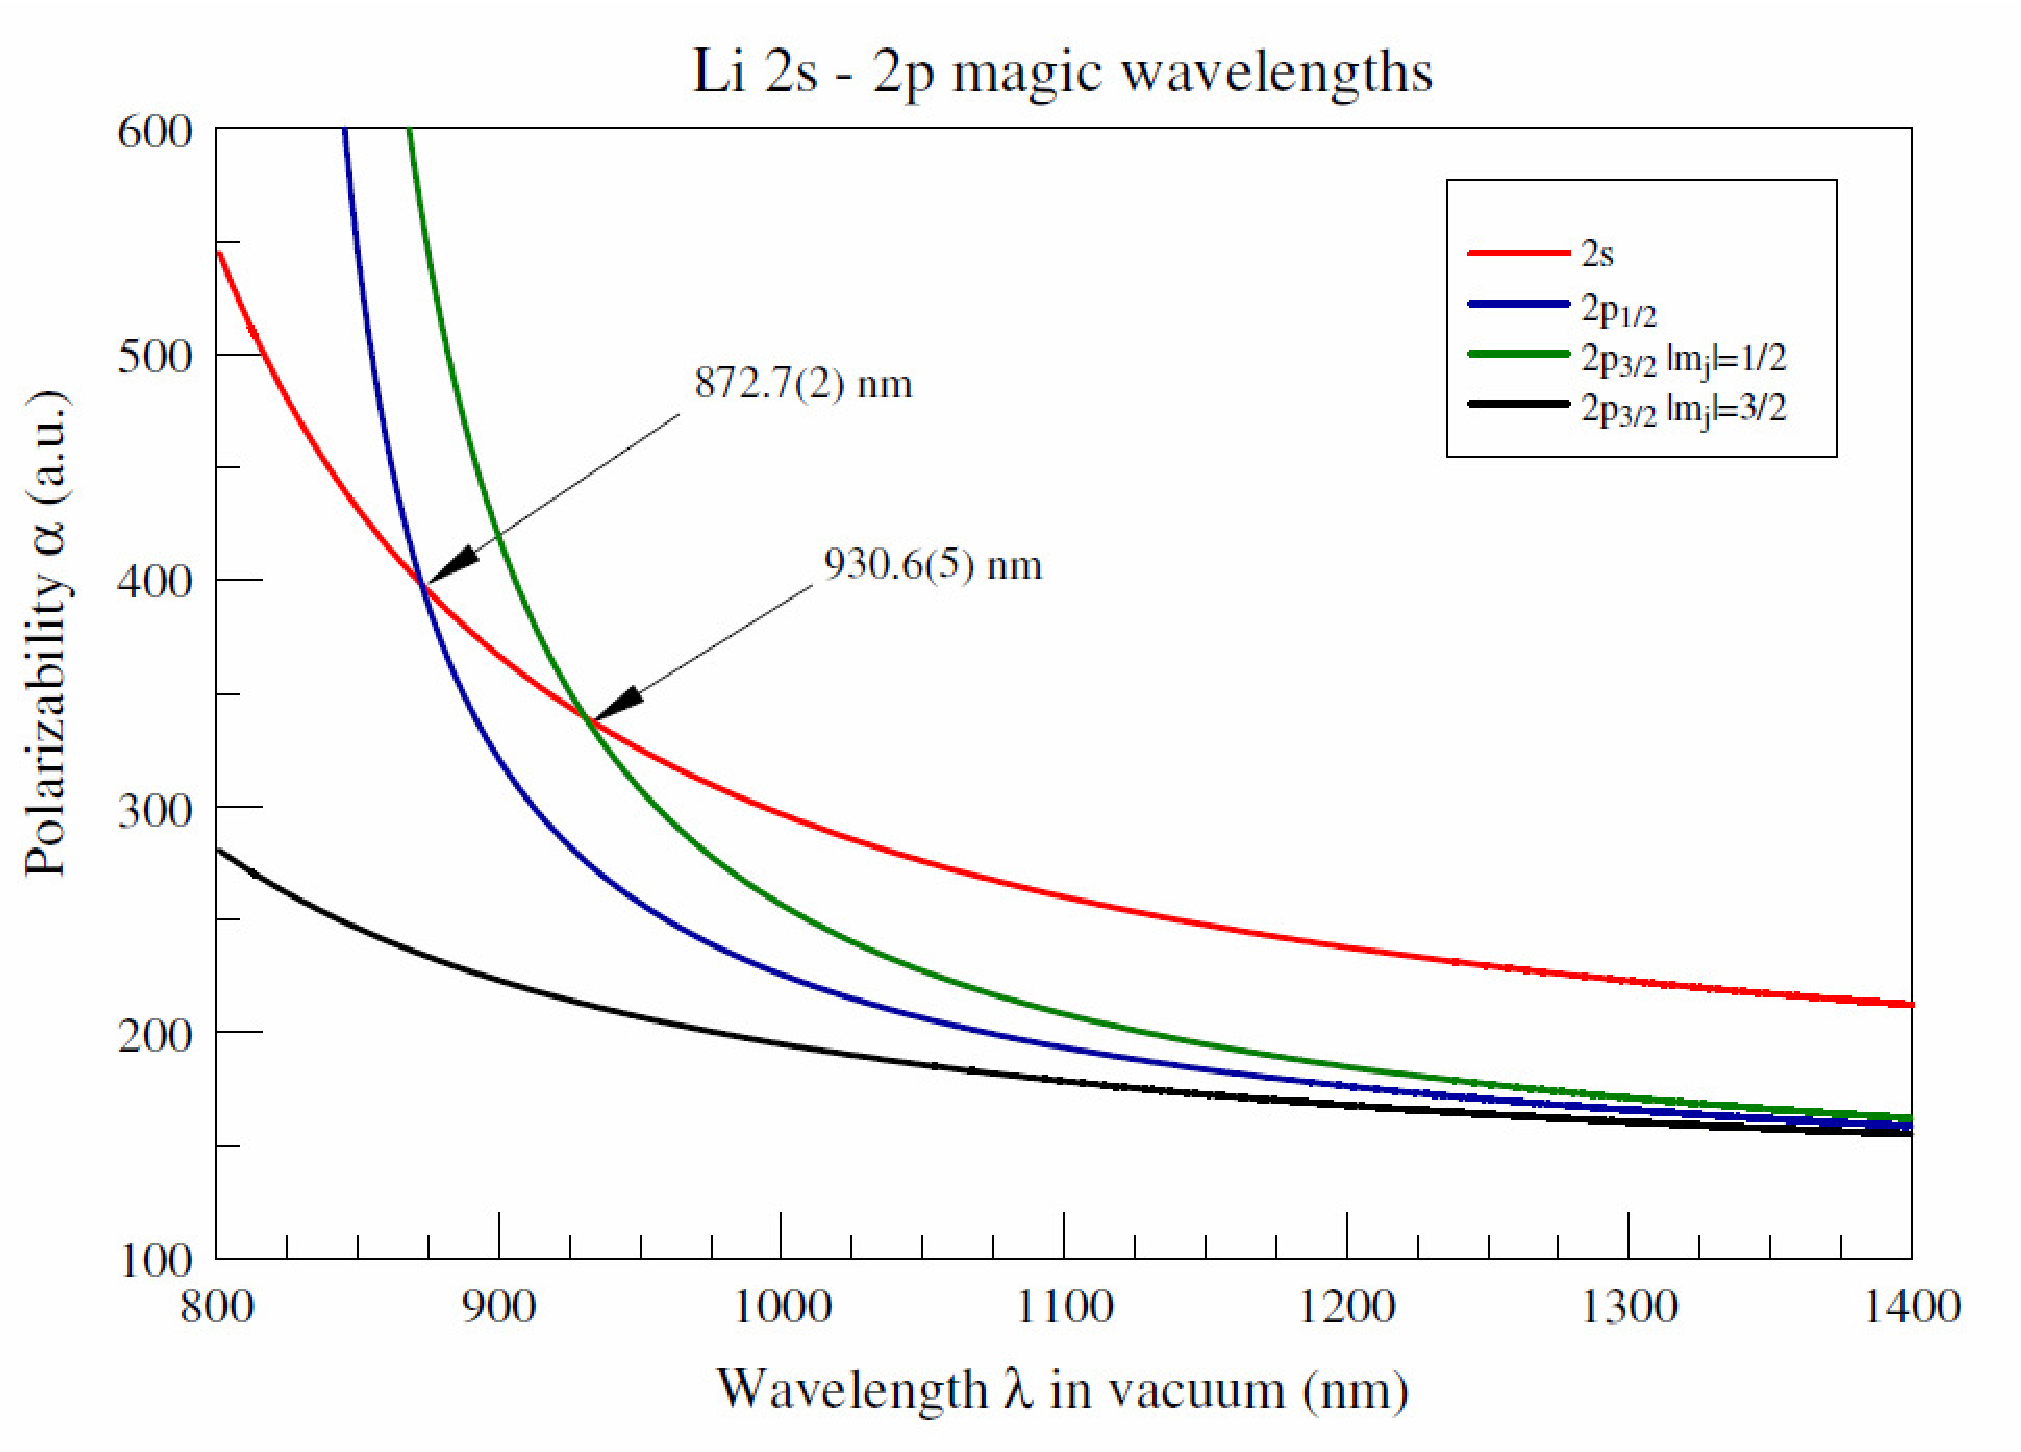
\includegraphics[width=0.7\textwidth]{../figures/safronova/2s2p.pdf}
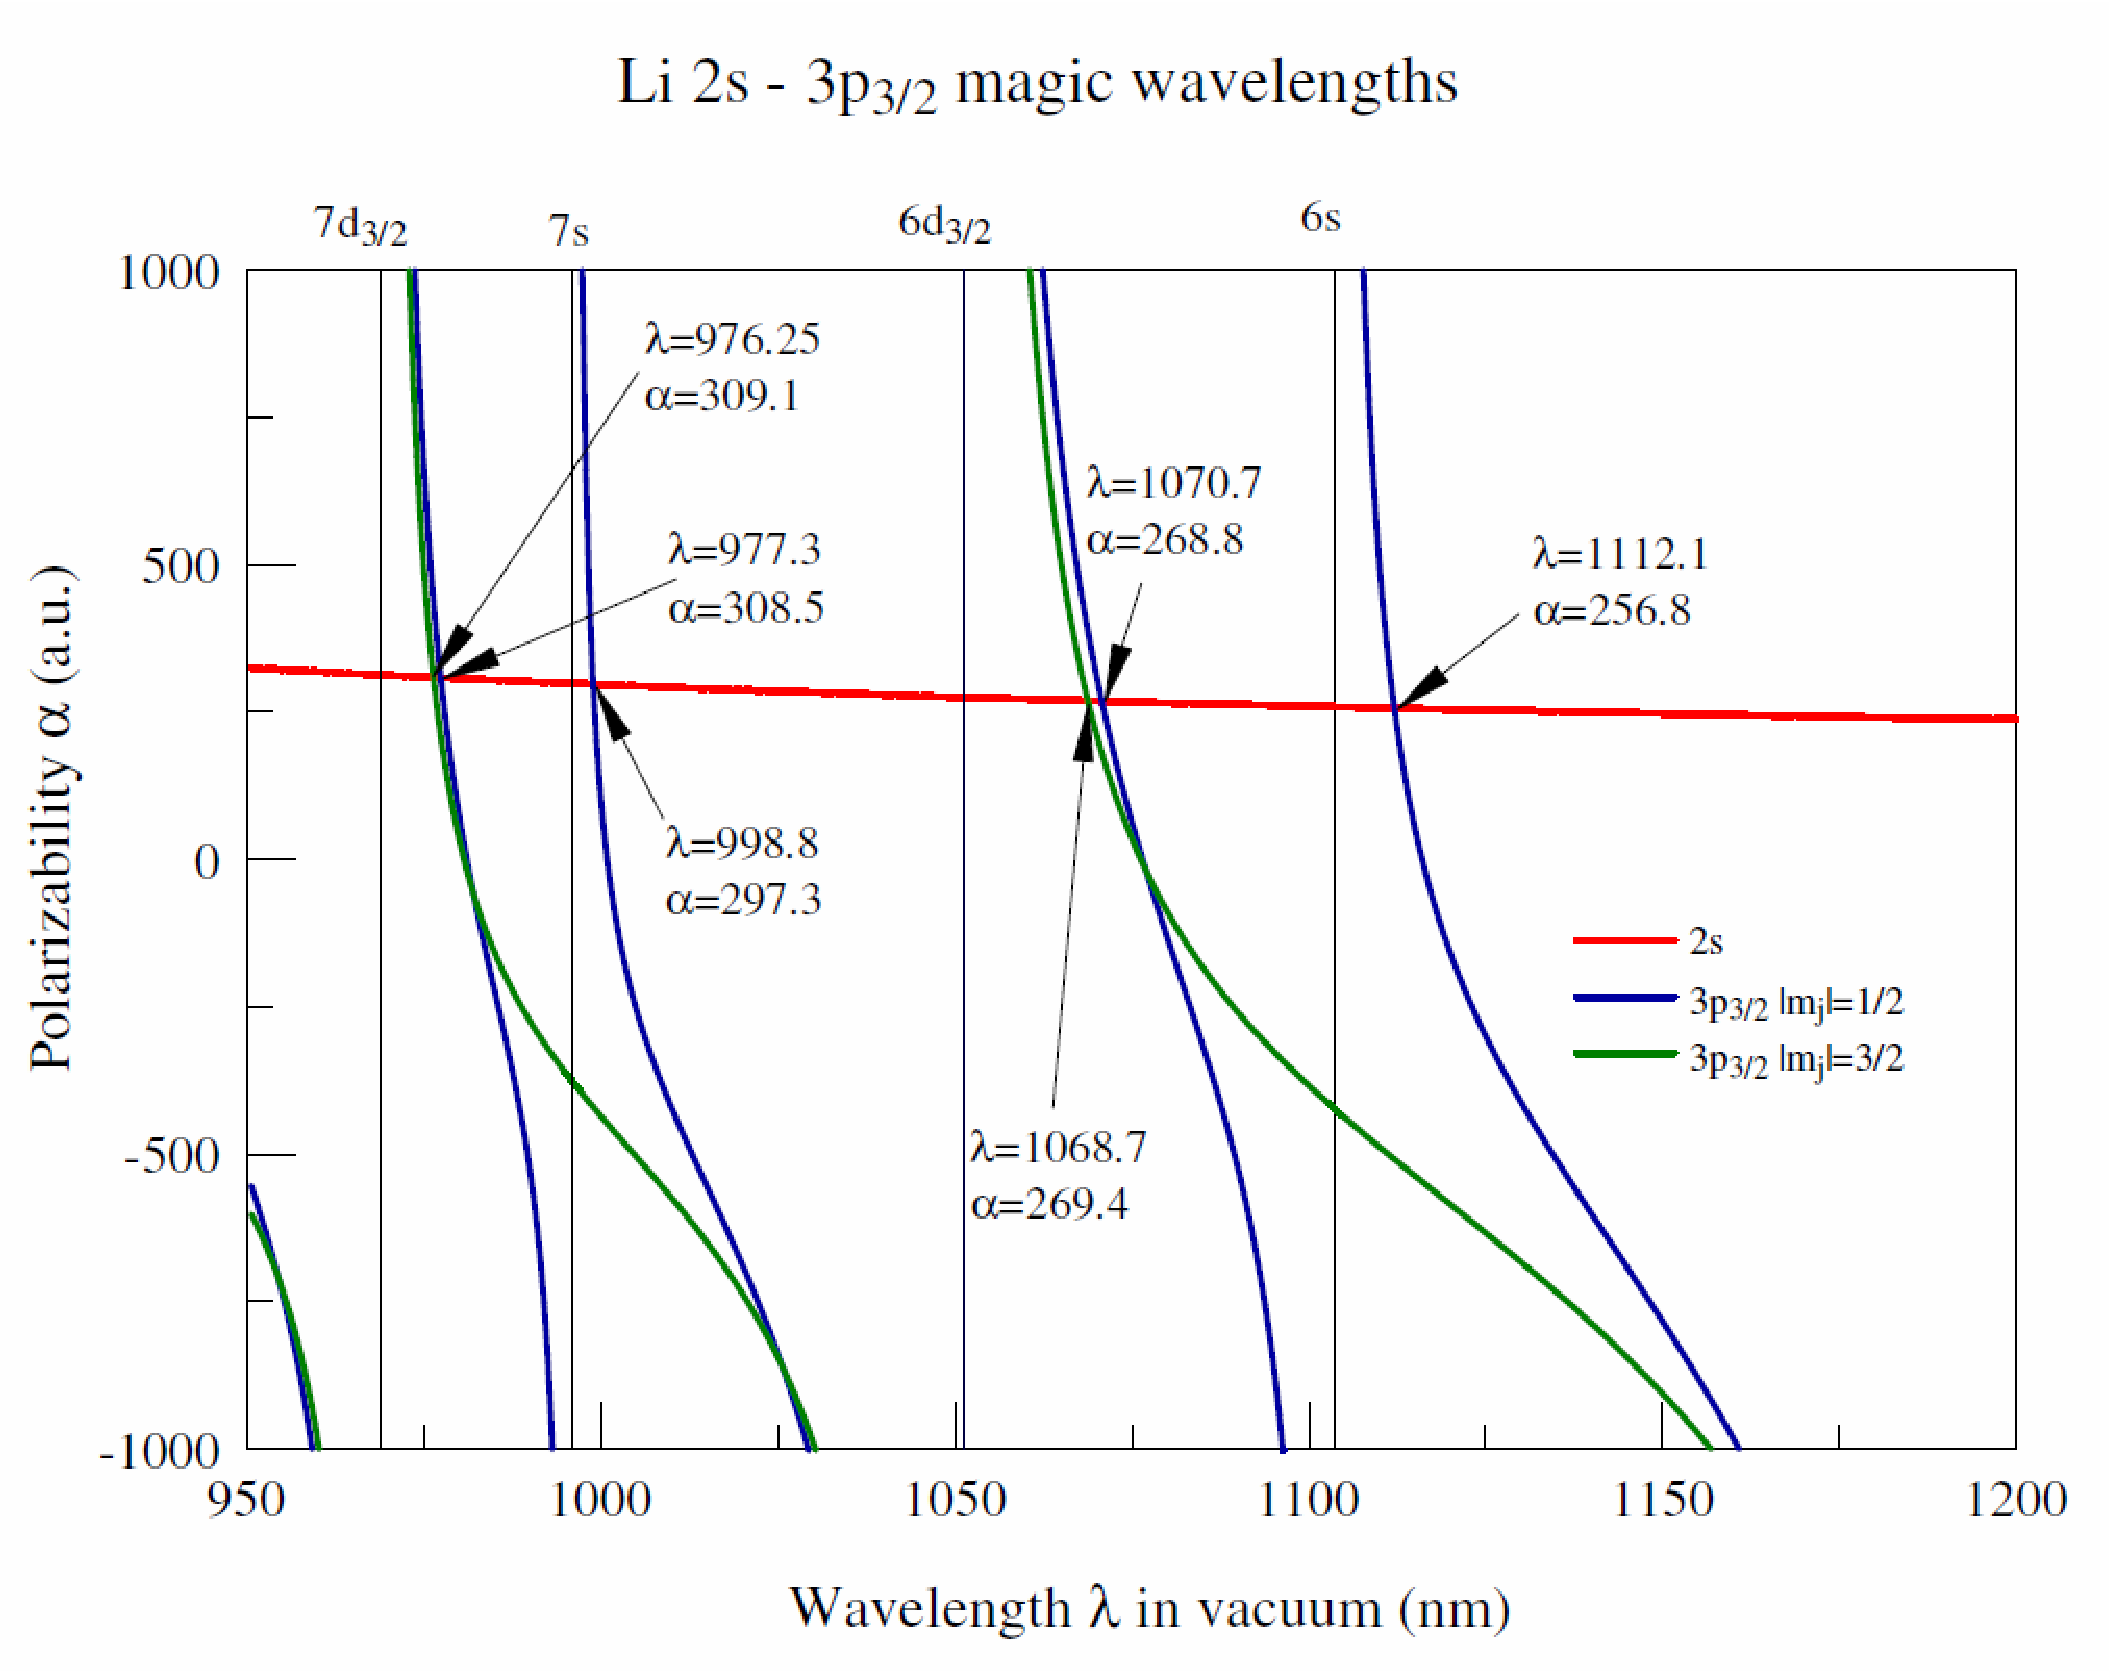
\includegraphics[width=0.7\textwidth]{../figures/safronova/2s3p.pdf}
\caption[Polarizabilities for 1070 nm light]{\small (Top) Polarizability in
atomic units for the $2S$ and $2P$ states. Magic wavelengths are indicated by
the arrows.   (Bot) Polarizability in atomic units of the $2S$ and $3P$ states.
The atomic units for polarizability can be converted to SI units
(C\,m$^{2}$\,V$^{-1}$) by multiplying by
1.648$\times10^{-41}$~\cite{Safronova2006,Safronova2010}.}
\label{fig:safronova} \end{figure} Figure~\ref{fig:lightshift}(a) shows how the
differential Stark shift  varies  as a function of wavelength near 1070~nm for
the intensity of our dipole trap.  Even a small AC Stark shift of the line
could be significant given the narrow linewidth of the UV transition.   We find
that to best load atoms to the trap we need to shift the UV cooling frequency
to the blue by approximately one linewidth compared to the frequency for
optimal performance of the UVMOT in free space.  \begin{figure}
\makebox[0.5\textwidth][l]{(a)}\makebox[0.5\textwidth][l]{(b)}
\begin{minipage}{0.5\linewidth} \centering
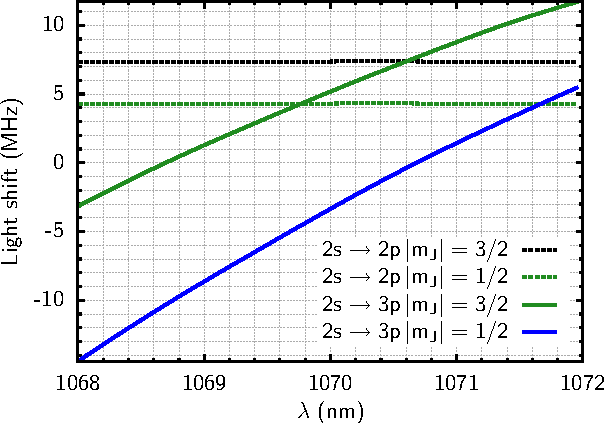
\includegraphics[width=0.9\textwidth]{../figures/safronova/diffpoleps.pdf}
\end{minipage} \begin{minipage}{0.5\linewidth} \centering
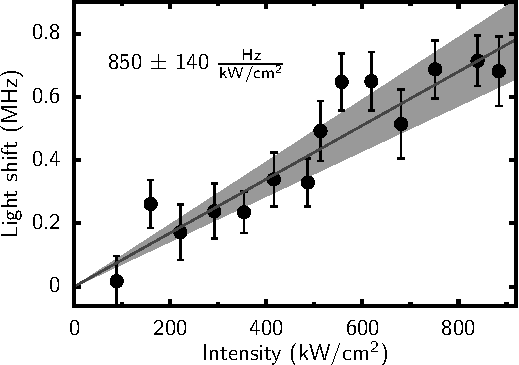
\includegraphics[width=\textwidth]{../figures/lightshift/lightshifteps.pdf}
\end{minipage} \caption[Differential AC Stark shift for 1070 nm light]{\small
(a) Differential AC Stark shift of the \red and \uv transitions as a function
of wavelength for an intensity of 910 kW/cm$^{2}$, calculation by M.~Safronova
(personal communication). The color code is the same as in
Fig.~\ref{fig:safronova}.  
(b) Differential AC Stark shift of the \uv transition
as a function of intensity of the optical trapping light at
$\lambda=1070\,\mathrm{nm}$.  The circles represent the center of a Gaussian fit of a loss
resonance and the error bars are 1 $\sigma$ statistical error of these fits.
The solid line is a linear fit to the resonance position with a slope of
$850(140) \,\mathrm{Hz/(kW/cm^{2})}$, where the error represents the
statistical uncertainty of the fit and a systematic uncertainty of 10\% on the
value of the trap intensity.  The gray shaded region indicates the error of the
linear fit. } \label{fig:lightshift} \end{figure}

We measured the differential AC Stark shift of the UV cooling transition  by
performing spectroscopy in the optical dipole trap.  The atoms are first cooled
to $T=3.5\,\mu$K by $6$~s of forced evaporation as shown in
Fig.~\ref{fig:evap}.  Following evaporation, the optical trap is adiabatically
ramped to various peak intensities, and the magnetic field is then quickly
ramped to zero where the atoms are illuminated by UV light with a frequency
tuned near the \twos{1/2}, $F=1/2$, $\rightarrow\,$\trep{3/2} transition.
Resonant excitation causes atoms to be optically pumped out of the $F=1/2$
ground state.  The population remaining in \two is subsequently measured by
absorption imaging.  Spectra are recorded at several trap intensities, and the
center of each is found by fitting to a Gaussian.  These resonance locations
are displayed as a function of peak intensity in Fig.  \ref{fig:lightshift}(b).
We find that at full trap depth, the UV transition is shifted to a 750 kHz
greater frequency than for free space.  This is consistent with our observation
that atoms are most efficiently loaded from the UV MOT when the UV laser
frequency is shifted to the blue by approximately one linewidth.  With this
detuning the temperature of atoms loaded into the optical trap is
$70\,\mu$K, close to the temperature in the MOT.  



%%%%%%%%%%%%%%%%%%%%%%%%%%%%%%%%%%%%%%%%%
%%%%%%%%%%%%%%%%%%%%%%%%%%%%%%%%%%%%%%%%% 
\chapter{Conclusion} 
\label{ch:conclusion}
%%%%%%%%%%%%%%%%%%%%%%%%%%%%%%%%%%%%%%%%%
%%%%%%%%%%%%%%%%%%%%%%%%%%%%%%%%%%%%%%%%% 

In this thesis I have described the first realization of narrow linewidth
cooling of \li atoms.  In conjunction with a 1070~nm optical dipole trap,
narrow linewidth cooling has proved to be an excellent tool for the creation of
a degenerate Fermi gas. The fact that the light shift in the 1070~nm trap is
small and to the blue ensures that laser cooling is effective throughout the
trap volume, providing an efficient way of loading the atoms from the narrow
line MOT into the trap.  After evaporation in the optical trap at 280~$a_{0}$,
we are able to reach numbers in  degenerate samples that only had been attained
before with much slower duty-cycle sympathetic cooling experiments.  

The fast and efficient production of degenerate Fermi gases provides an
excellent starting point for future experiments.  We are currently implementing
a three dimensional optical lattice to study the rich physics of the
Fermi-Hubbard model.  \li atoms in an optical lattice with controllable
interactions can be described by the Fermi-Hubbard Hamiltonian for a two-spin
component Fermi gas.  This Hamiltonian is relevant for understating strongly
correlated electron systems and in particular it may capture the essential
physics responsible for high-$T_{c}$ superconductivity~\cite{Anderson2002}

Our next milestone is to search for evidence of the antiferromagnetically
ordered N\`{e}el state, that is known to occur in the normal phase of the
Fermi-Hubbard model at half-filling.  We will try to detect the
antiferromagnetic state by use of a Bragg scattering
technique~\cite{Ted2010}.  The geometry of Apparatus3 was specifically chosen
to accommodate the angles necessary for the detection of antiferromagnetism
with Bragg scattering. After four long years of building up, Apparatus3 is
finally approaching the physics which it was meant to study. 


% if appendices, then
%\appendix
%\chapter{Appendix}


% if Biographical sketch then
%\begin{biosketch}
%I was kissed by a donkey when I was 5..... and text and more text and even more text, lots of text, here and there, more and more text, with more and more descriptions of text, blah etc blah et
%\end{biosketch}

\bibliographystyle{osa}
% Other options for the bibliographystyle are listed below
%\bibliographystyle{unsrt}
%\bibliographystyle{unsrtnat}
%\bibliographystyle{apsrev}
\bibliography{pmd}

\end{document}

